\chapter{ Chapitre 4 : Sprint 1 \centering
    "Gestion des Utilisateurs"  }
\begin{spacing}{1.2}
\minitoc
\thispagestyle{MyStyle}
\end{spacing}
\newpage
\begin{sloppypar} 
\section{Introduction}
\vspace{-4mm}
Dans notre premier sprint Nous nous concentrons sur la création de comptes, l'authentification, la gestion des utilisateurs, et la réinitialisation des mots de passe. Notre objectif : mettre en place un système robuste pour permettre aux utilisateurs de s'inscrire, de se connecter en toute sécurité et de récupérer leur mot de passe en cas d'oubli. En travaillant ensemble, nous fournirons une solution fiable et conviviale pour nos utilisateurs.
\vspace{-7mm}
\section{Backlog du sprint}
\vspace{-7mm}
Le backlog de gestion des utilisateurs présente une série de tâches et de fonctionnalités destinées à faciliter la gestion des comptes des utilisateurs dans notre application.Ces éléments incluent des fonctionnalités telles que la création de compte, l'authentification, la gestion des profils, la réinitialisation des mots de passe et d'autres fonctionnalités liées à la gestion des utilisateurs. 

\begin{table}[h]
\centering
\begin{tabular}{|p{10cm}|p{2cm}|p{2.5cm}|}
\hline
\textbf{Tâches} & \textbf{Priorité} & \textbf{Période/jour} \\
\hline
En tant qu’un étudiant, je peux créer un compte dans l’application mobile. & Élevée & 5 jours \\
\hline
En tant qu’un utilisateur (admin et étudiant), je peux m’authentifier dans l’application mobile. & Moyenne & 3 jours \\
\hline
En tant qu’un administrateur, je peux m’authentifier à l’application web. & Moyenne & 4 jours \\
\hline
En tant qu’un administrateur, je peux supprimer les étudiants depuis l’application web. & Moyenne & 3 jours \\
\hline
En tant qu'un utilisateur, je peux modifier les données de mon compte. & Moyenne & 4 jours \\
\hline
En tant qu'un utilisateur, je peux réinitialiser mon mot de passe sur la partie mobile. & Moyenne & 3 jours \\
\hline
\end{tabular}
\caption{Tableau de Backlog de produit Sprint 1}
\end{table}

\vspace{-1.2cm}
\section {Analyse et spécification des besoins}
\vspace{-4mm}
\section {Diagramme de cas d'utilisation detaillé}
\vspace{-4mm}
Afin de mieux comprendre la structure de notre système, nous avons utilisé un diagramme de cas d'utilisations qui est présenté ci-dessous [17].

\begin{figure}[H]%
    \center%
    \setlength{\fboxsep}{5pt}%
    \setlength{\fboxrule}{0.5pt}%
    \fbox{
    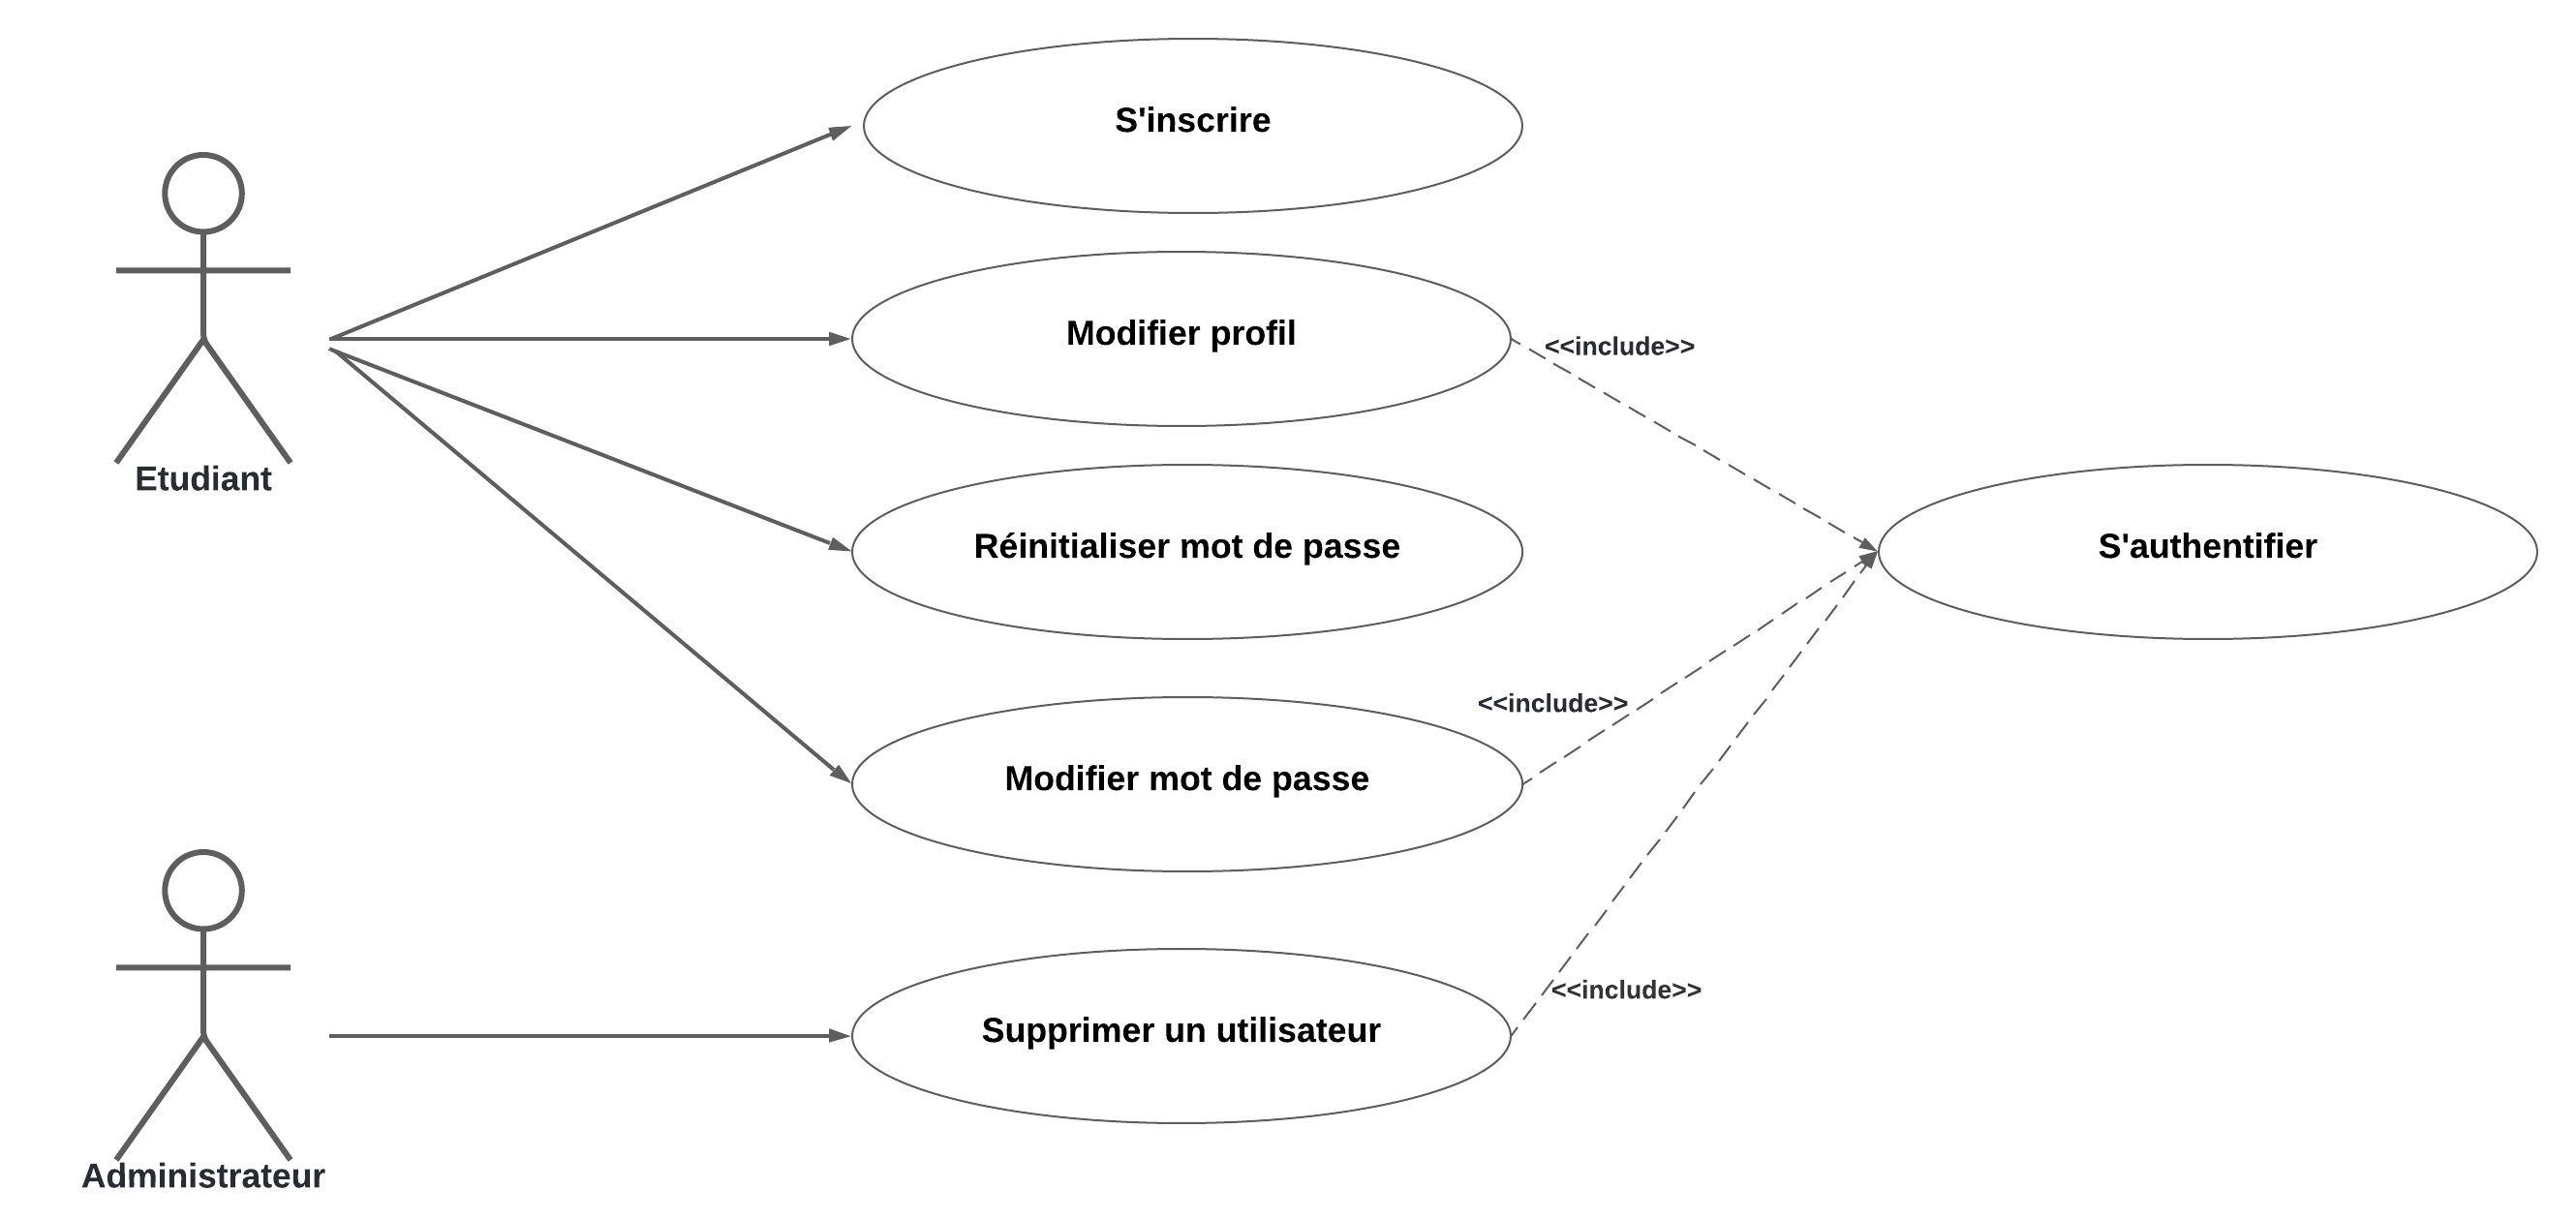
\includegraphics[height=9cm,width=13cm]{images/AAAUseCasesAuthentification.png}%
    }
    \caption{Figure du Diagramme de cas d'utilisation sprint 1}
\end{figure}

\vspace{-1.3cm}
\subsection{Description textuelle du cas d’utilisation « S'inscrire »}
\vspace{-3mm}
Le diagramme ci-dessous illustre le processus d'inscription dans la section mobile de notre application. Cette inscription est une étape essentielle pour accéder aux fonctionnalités de l'application.

\begin{table}[h]
\centering
\begin{tabular}{|p{3cm}|p{12cm}|}
\hline
\textbf{Cas d'utilisation } & S’inscrire  \\
\hline
\textbf{Acteurs} & Étudiant, Admin \\
\hline
\textbf{Précondition} & Non inscrit et non connecté \\
\hline
\textbf{Postcondition} & Inscription validée et succès d‘accès \\
\hline
\textbf{Scénario nominal} & 
\begin{enumerate}
    \item Le système affiche la page de SignUp.
    \item L’acteur saisit son Email et son mot de passe.
    \item L’acteur appuie sur le bouton « S’inscrire ».
    \item L'utilisateur remplit ses informations personnelles.
\end{enumerate} \\
\hline
\textbf{Scénario alternatif} & 
\begin{enumerate}
    \item L’acteur saisit son Email et son mot de passe.
    \item Le système vérifie si l'Email existe déjà.
    \item Si l'Email existe déjà, le système affiche un message d’erreur informant que le compte existe déjà.
\end{enumerate} \\
\hline
\textbf{Exceptions} &  Un champ est vide. Le système affiche un message d’erreur informant qu'il y a des champs à remplir. \\
\hline
\end{tabular}
\caption{Description du cas d’utilisation « S'inscrire »}
\end{table}


\vspace{-9mm}
\subsection{Description textuelle du cas d’utilisation « S’authentifier »}
\vspace{-4mm}
Le diagramme suivant décrit la phase d’authentification dans la partie mobile de notre application. L'authentification est une étape cruciale pour accéder aux fonctionnalités de notre application.
\vspace{5mm}
\begin{table}[h]
\centering
\begin{tabular}{|p{3cm}|p{12cm}|}
\hline
\textbf{Cas d'utilisation} & S’authentifier  \\
\hline
\textbf{Acteurs} & Étudiant, Admin \\
\hline
\textbf{Précondition} & Déjà inscrit mais non connecté \\
\hline
\textbf{Postcondition} & Authentification validée et succès d‘accès \\
\hline
\textbf{Scénario nominal} & 
\begin{enumerate}
    \item Le système affiche la page de connexion.
    \item L’acteur saisit son Email et son mot de passe.
    \item L’acteur appuie sur le bouton « S’identifier ».
    \item Le système vérifie la validité des informations fournies. Si les informations sont incorrectes, alors appel de l’exception.
\end{enumerate} \\
\hline
\textbf{Scénario alternatif} & 
\begin{enumerate}
    \item L’acteur clique sur « Mot de passe oublié ».
    \item Le système affiche une page de récupération de mot de passe.
    \item L’acteur saisit son Email et appuie sur « Envoyer ».
    \item Le système envoie un Email de récupération à l’acteur.
    \item L’acteur clique sur le lien de récupération dans l'Email et saisit un nouveau mot de passe.
    \item Le système enregistre le nouveau mot de passe et affiche une confirmation de succès.
\end{enumerate} \\
\hline
\textbf{Exception} & 
\begin{enumerate}
    \item Login et/ou mot de passe incorrect(s).
    \item Le système affiche un message d’erreur informant l’utilisateur que son login ou mot de passe est incorrect.
\end{enumerate} \\
\hline
\end{tabular}
\caption{Description du cas d’utilisation « S'authentifier »}
\end{table}

\vspace{-1cm}
\subsection{Description textuelle du cas d’utilisation « Modifier le profil »}
\vspace{-4mm}
Le diagramme suivant présente le processus de modification de profil dans la partie mobile de notre application. Cette étape implique deux acteurs : l'étudiant et l'admin.
\begin{table}[h]
\centering
\begin{tabular}{|p{3cm}|p{12cm}|}
\hline
\textbf{Cas d'utilisation } & Modifier le profil  \\
\hline
\textbf{Acteurs} & Etudiant, Admin \\
\hline
\textbf{Précondition} & Acteurs authentifiés \\
\hline
\textbf{Postcondition} & Modification validée \\
\hline
\textbf{Scénario nominal} &
\begin{enumerate}
    \item Le système affiche l’interface de modification.
    \item L’acteur saisit ses informations personnelles.
    \item Le système modifie le profil.
    \item Le système affiche un message de succès.
\end{enumerate} \\
\hline
\end{tabular}
\caption{Description du cas d’utilisation « Modifier le profil »}
\end{table}


\vspace{0cm}
\subsection{Description textuelle du cas d’utilisation « Modifier mot de passe »}
\vspace{-4mm}
Le diagramme ci-dessous présente le déroulement de la modification du mot de passe dans la section mobile de notre application. Deux acteurs doivent participer à cette étape : l'étudiant et l'admin.

\begin{table}[h]
\centering
\begin{tabular}{|p{3cm}|p{12cm}|}
\hline
\textbf{Cas d'utilisation } & Modifier mot de passe  \\
\hline
\textbf{Acteurs} & Etudiant, Admin \\
\hline
\textbf{Précondition} & Acteurs authentifiés \\
\hline
\textbf{Postcondition} & Mot de passe modifié \\
\hline
\textbf{Scénario nominal} &
\begin{enumerate}
    \item L’acteur clique sur le bouton « modifier le mot de passe ».
    \item Le système affiche l’interface de modification de mot de passe.
    \item L’acteur saisit et confirme son nouveau mot de passe. Si le mot de passe est invalide .
    \item Le système affiche un message de succès.
\end{enumerate} \\
\hline
\textbf{Exception } & Mot de passe vide ou ne répond pas aux exigences. \\
& Le système affiche un message d’erreur. \\
\hline
\end{tabular}
\caption{Description du cas d’utilisation « Modifier mot de passe »}
\end{table}

\vspace{-1.2cm}
\section{Diagramme de séquence }
\vspace{-4mm}

Les diagrammes de séquence décrivent de manière séquentielle les interactions entre l'utilisateur et le système lors de la gestion des utilisateurs.

\vspace{-9mm}
\subsection{Diagramme de séquence « S’inscrire »}
\vspace{-4mm}
Ce diagramme de séquence montre le processus par lequel un utilisateur s'inscrit dans un système. Il met en évidence les interactions entre l'utilisateur et le système nécessaires pour finaliser l'inscription.
\vspace{-4mm}
\begin{figure}[H]%
    \center%
    \setlength{\fboxsep}{5pt}%
    \setlength{\fboxrule}{0.5pt}%
    \fbox{
    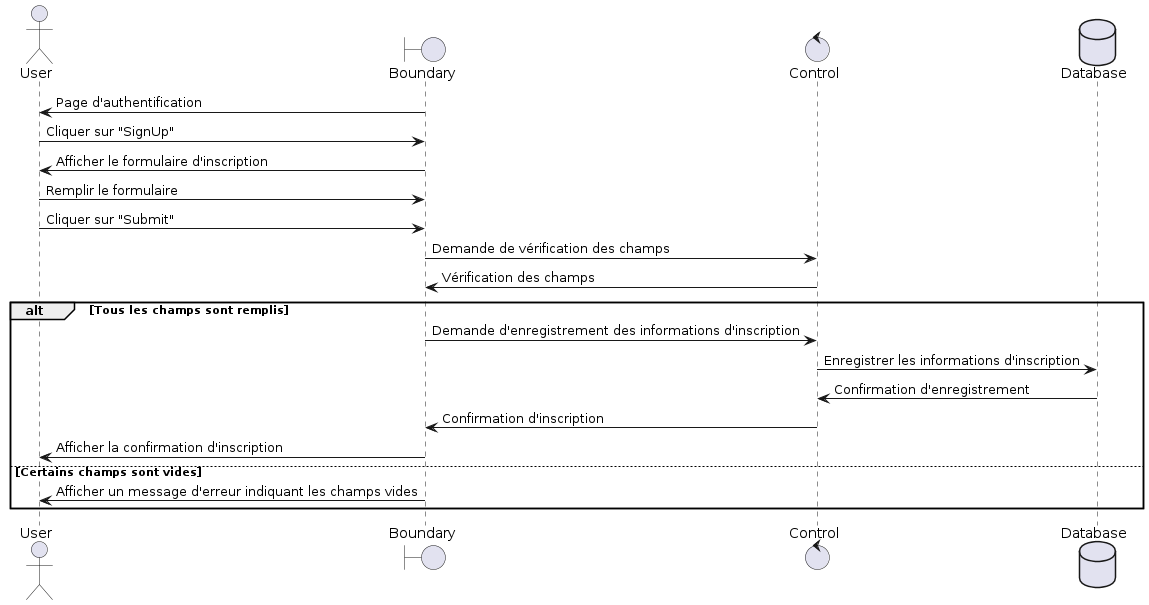
\includegraphics[height=8cm,width=15cm]{images/ffsignupp.png}%
    }
    \caption{Figure du Diagramme de sequence «s'inscrire»  }
\end{figure}
\vspace{-1.3cm}
\subsection{Diagramme de séquence « S’authentifier »}
\vspace{-4mm}
Ce diagramme de séquence illustre le processus d'authentification d'un utilisateur dans un système. Il décrit les interactions entre l'utilisateur et le système lors de la tentative de connexion avec un email et un mot de passe.
\vspace{-4mm}
\begin{figure}[H]%
    \center%
    \setlength{\fboxsep}{5pt}%
    \setlength{\fboxrule}{0.5pt}%
    \fbox{
    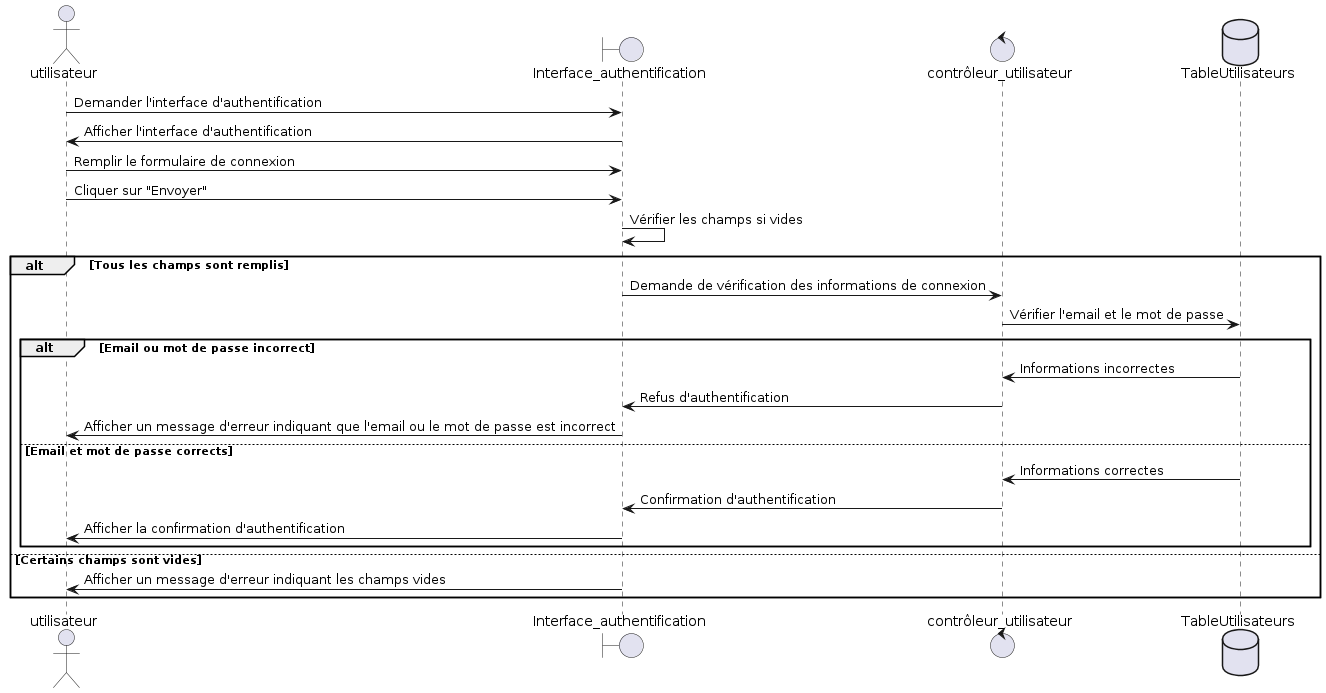
\includegraphics[height=10cm,width=15cm]{images/ffffloginX.png}%
    }
    \caption{Figure du Diagramme de sequence « s'authentifier » }
\end{figure}
\vspace{-1.3cm}
\subsection{Diagramme de séquence « Changer mot de passe »}
\vspace{-4mm}
Ce diagramme de séquence décrit le processus par lequel un utilisateur change son mot de passe dans un système. Il montre en détail les interactions entre l'utilisateur et le système nécessaires pour accomplir cette tâche.
\begin{figure}[H]%
    \center%
    \setlength{\fboxsep}{5pt}%
    \setlength{\fboxrule}{0.5pt}%
    \fbox{
    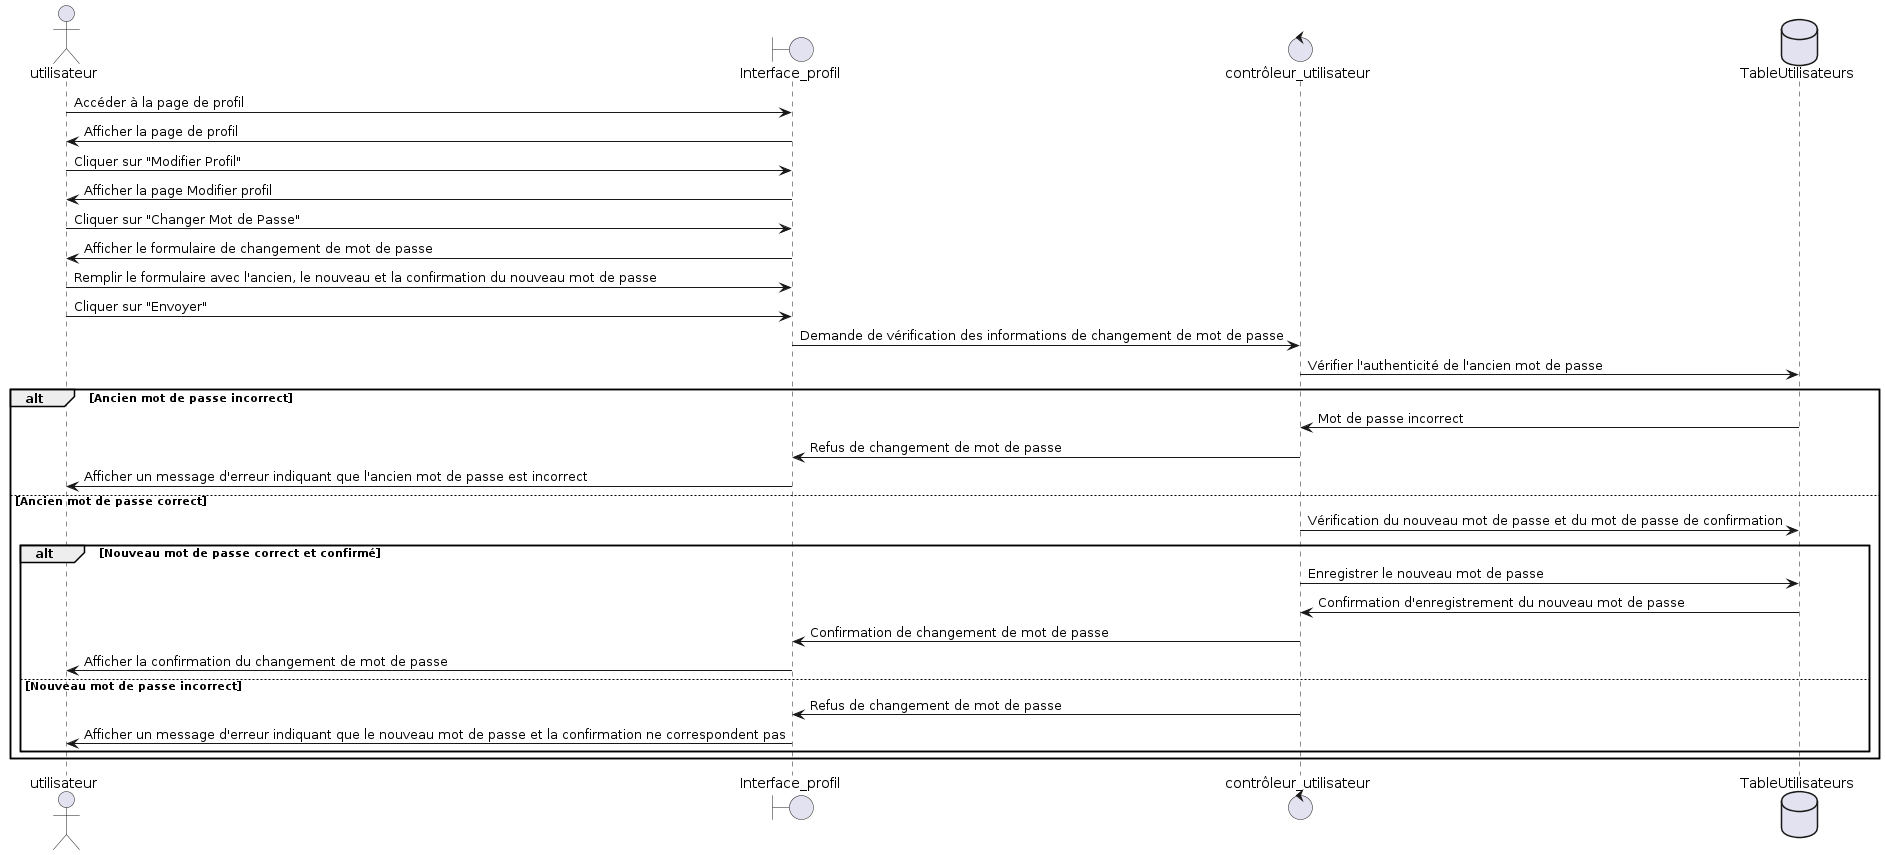
\includegraphics[height=15cm,width=15cm]{images/ffchangermotdepasseee.png}%
    }
    \caption{Figure du Diagramme de sequence «Changer mot de passe» }
\end{figure}
\vspace{-1.2cm}
\section{Diagramme de classes}
\vspace{-4mm}
Le diagramme de classes est un élément principal de conception d’un logiciel, c’est un modèle représentant la structure du système à concevoir. Le diagramme de classes est un schéma utilisé pour présenter les classes et les différentes relations. 
\begin{figure}[H]%
    \center%
    \setlength{\fboxsep}{5pt}%
    \setlength{\fboxrule}{0.5pt}%
    \fbox{
    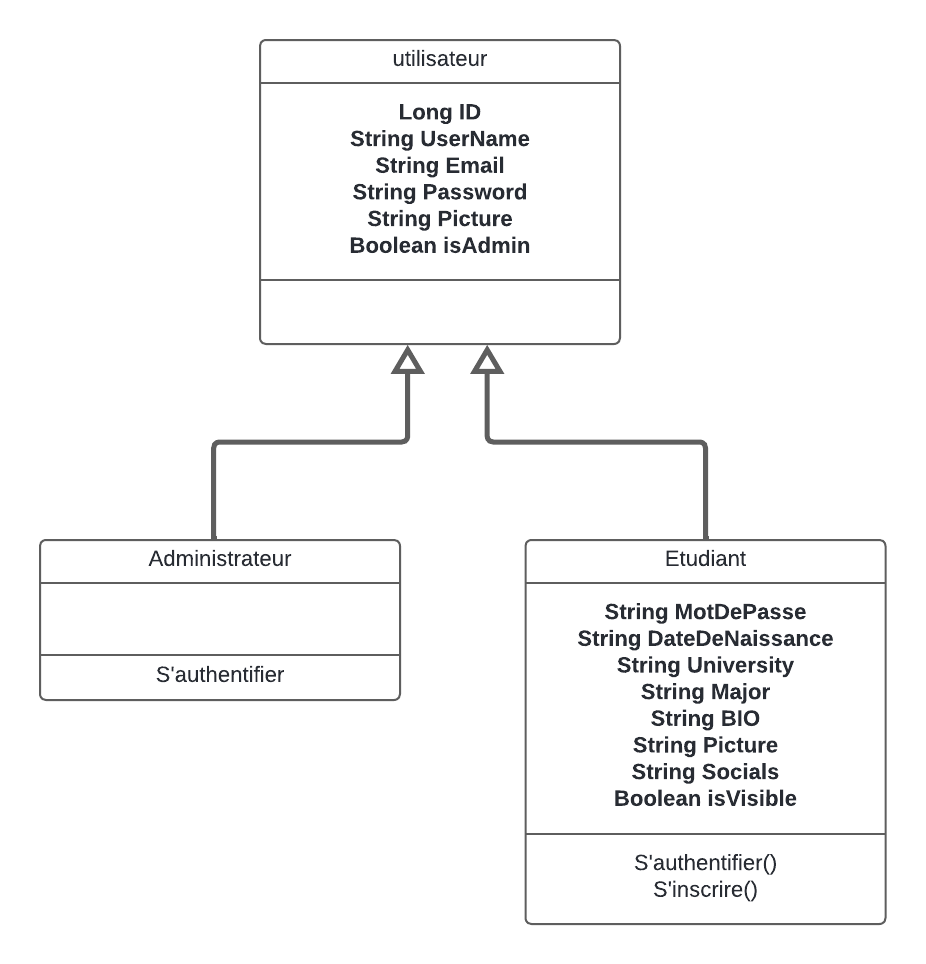
\includegraphics[height=17cm,width=15cm]{images/AAAAuthentification.png}%
    }
    \caption{Figure du Diagramme de classes Sprint 1}
\end{figure}
\vspace{-1.5cm}
\section{Réalisation }
\vspace{-4mm}
La partie de réalisation représente la dernière phase du cycle de développement d’un sprint. Elle permet de présenter les résultats obtenus lors de l’étape de développement afin d’assurer et de garantir une version de qualité.
\vspace{-7mm}
\subsection{Authentification}
\vspace{-3mm}
L’interface d’authentification, c’est la première interface vue par l’utilisateur.
\begin{figure}[H]%
    \center%
    \setlength{\fboxsep}{5pt}%
    \setlength{\fboxrule}{0.5pt}%
    \fbox{
    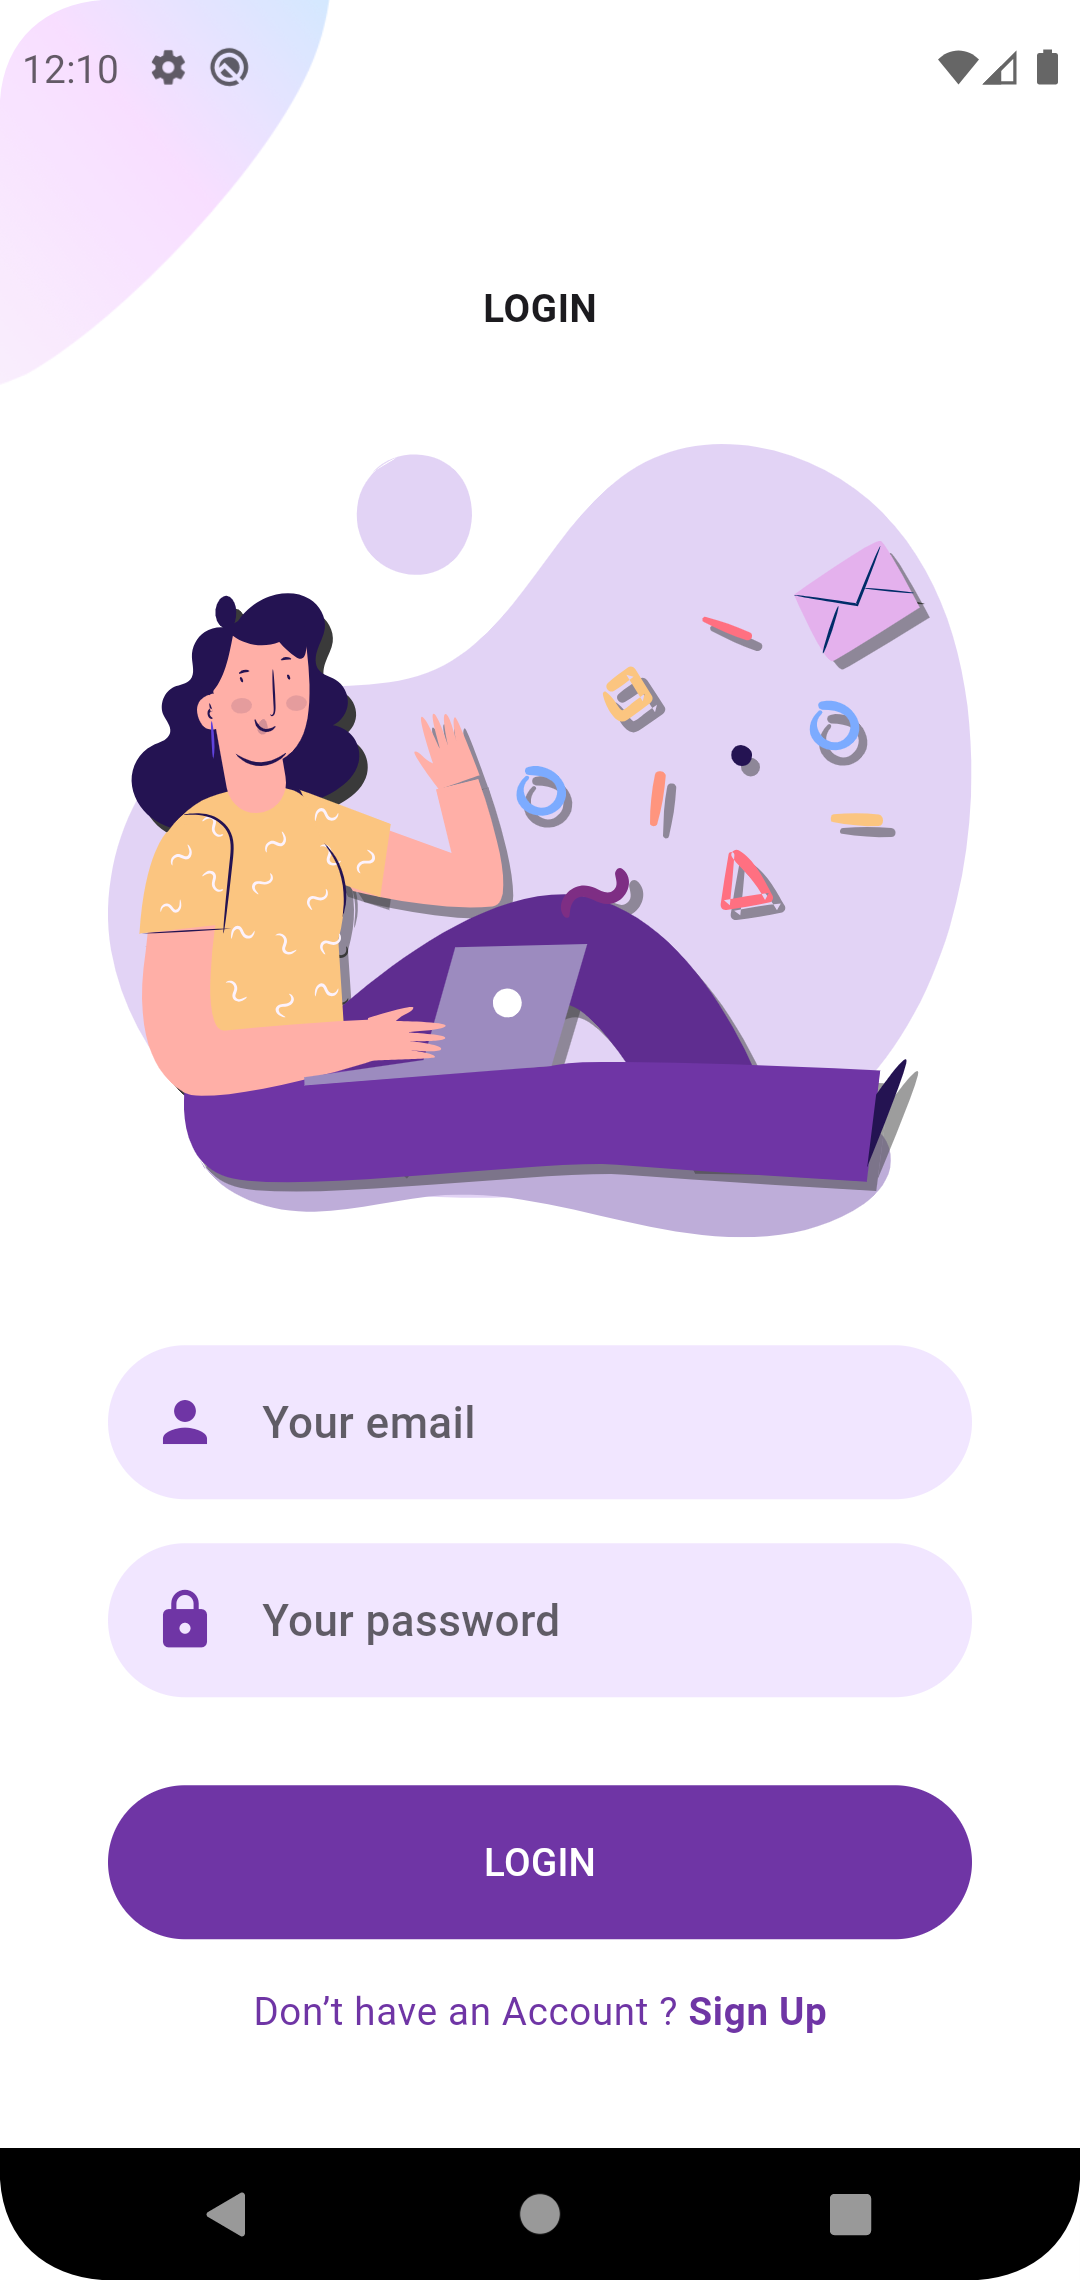
\includegraphics[height=9.5cm,width=7cm]{images/loginPage.png}%
    }
    \caption{Interface Login mobile}
\end{figure}
\vspace{-1.2cm}
\subsection{Authentification web}
\vspace{-4mm}
L’interface d’authentification pour la partie web, c’est la première interface vue par l’admin.
\vspace{-6mm}
\begin{figure}[H]%
    \center%
    \setlength{\fboxsep}{5pt}%
    \setlength{\fboxrule}{0.5pt}%
    \fbox{
    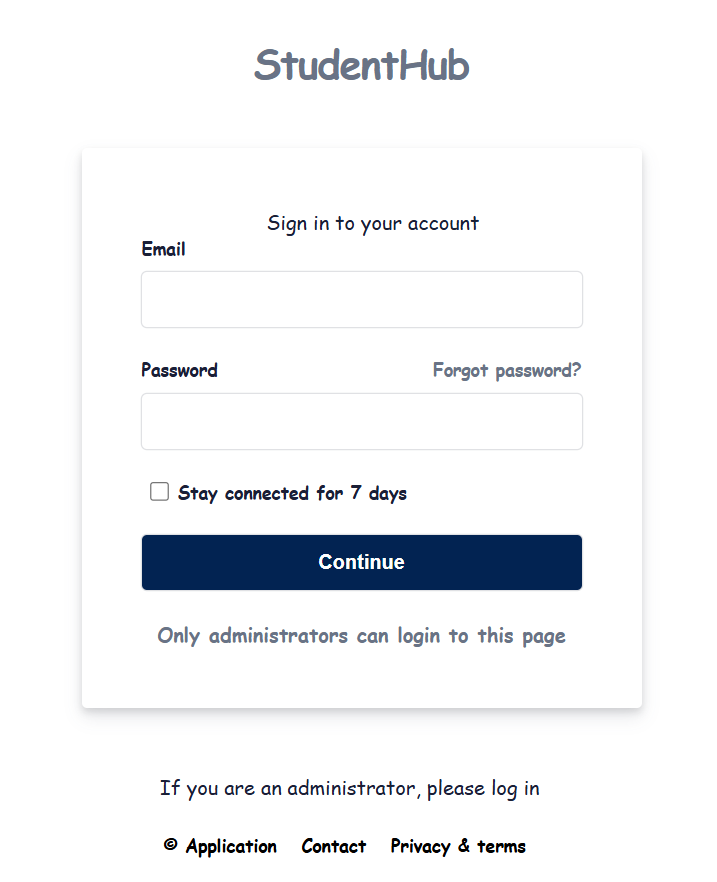
\includegraphics[height=9.5cm,width=12cm]{images/AdminLoginPage.png}%
    }
    \caption{Interface Login web }
\end{figure}

\subsection{Inscription}
\vspace{-4mm}
La page d'inscription permet aux nouveaux utilisateurs de créer leur compte facilement.
\begin{figure}[H]
    \centering

    \begin{subfigure}{0.45\textwidth}
        \centering
        \setlength{\fboxsep}{5pt}%
        \setlength{\fboxrule}{0.5pt}%
        \fbox{
            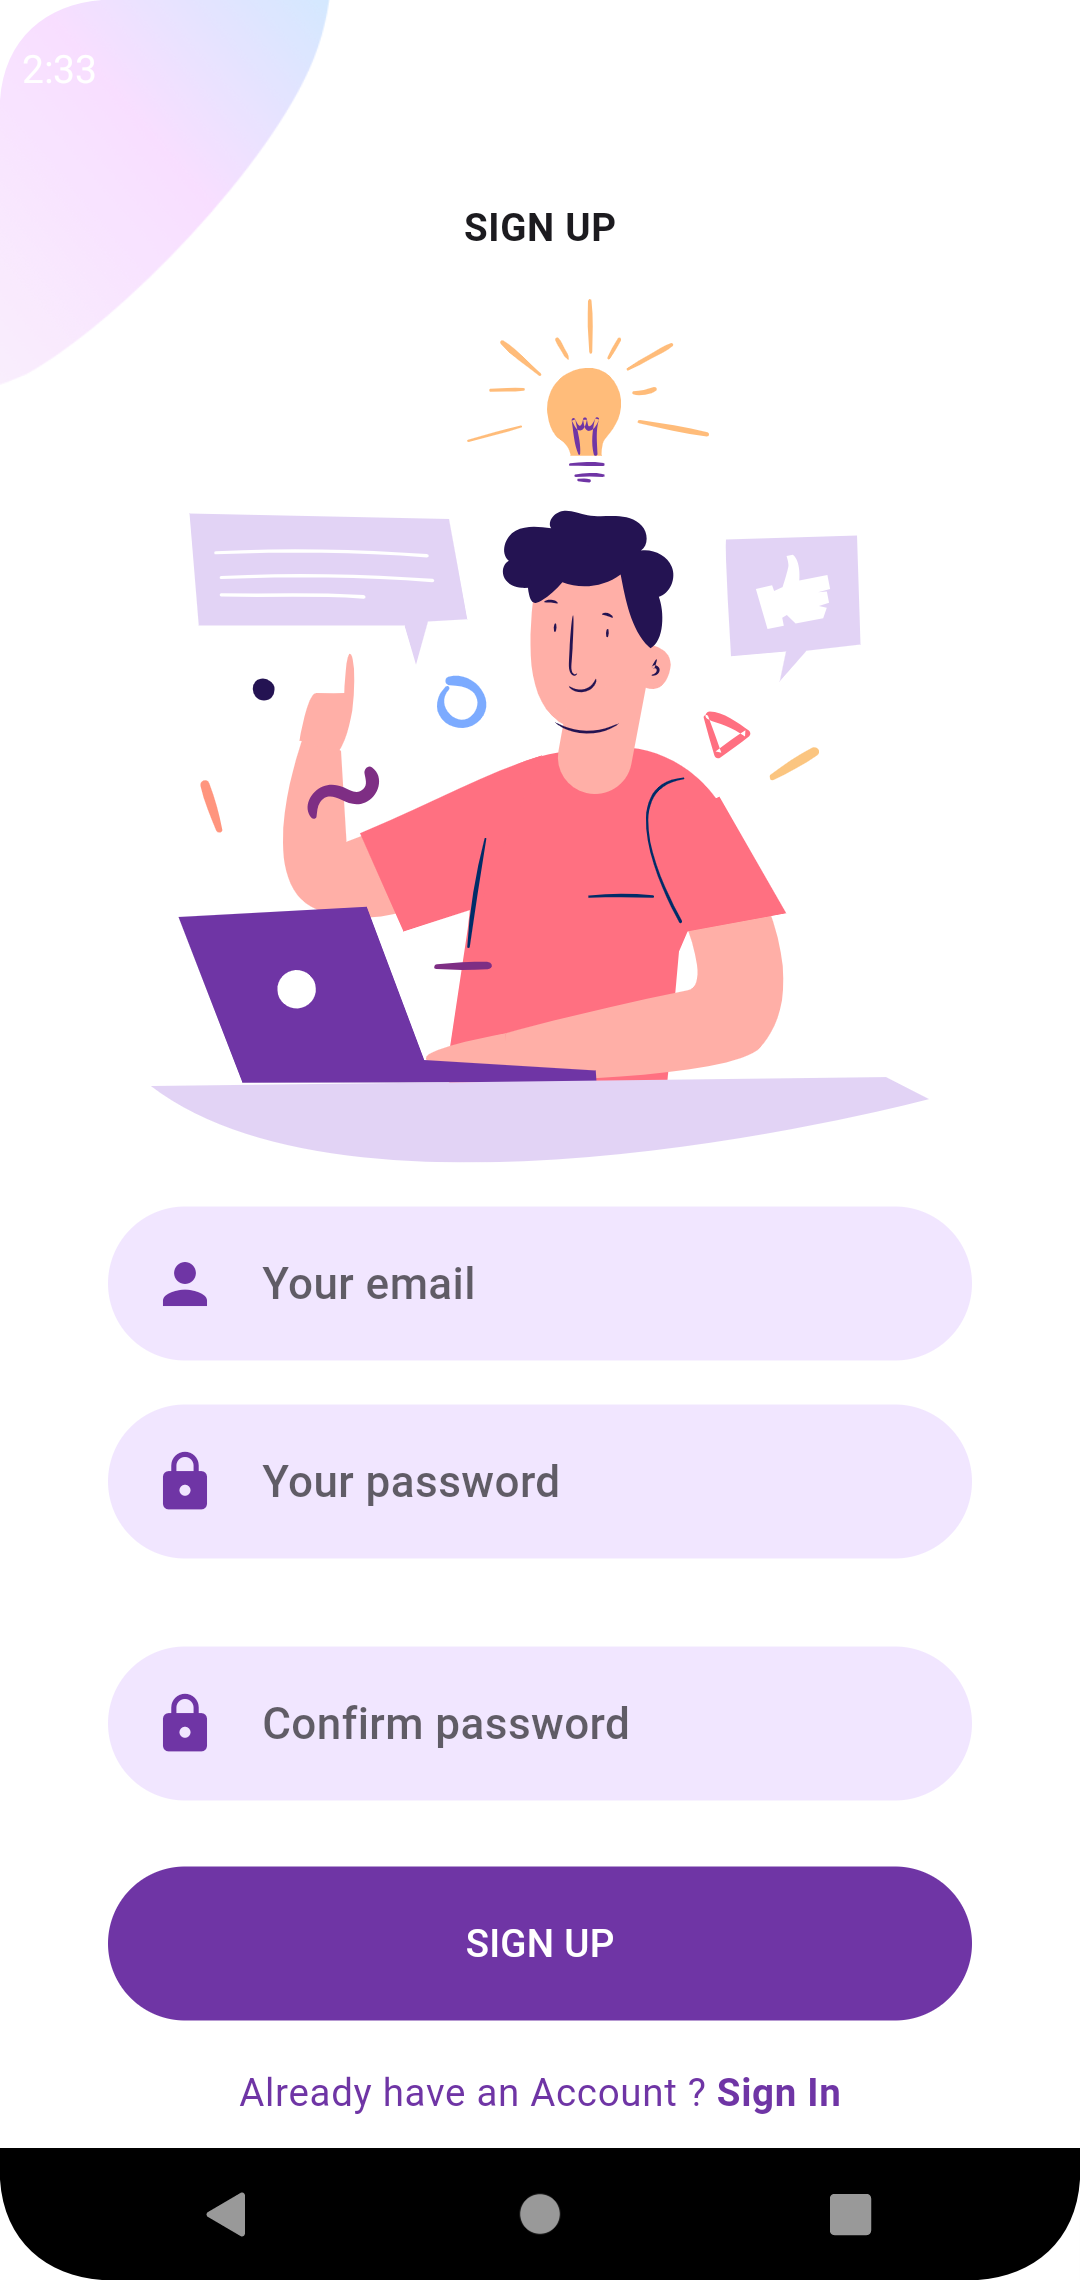
\includegraphics[height=9.5cm,width=7cm]{images/SignUpPage.png}
        }
        \label{fig:first}
    \end{subfigure}
    \hfill
    \begin{subfigure}{0.45\textwidth}
        \centering
        \setlength{\fboxsep}{5pt}%
        \setlength{\fboxrule}{0.5pt}%
        \fbox{
            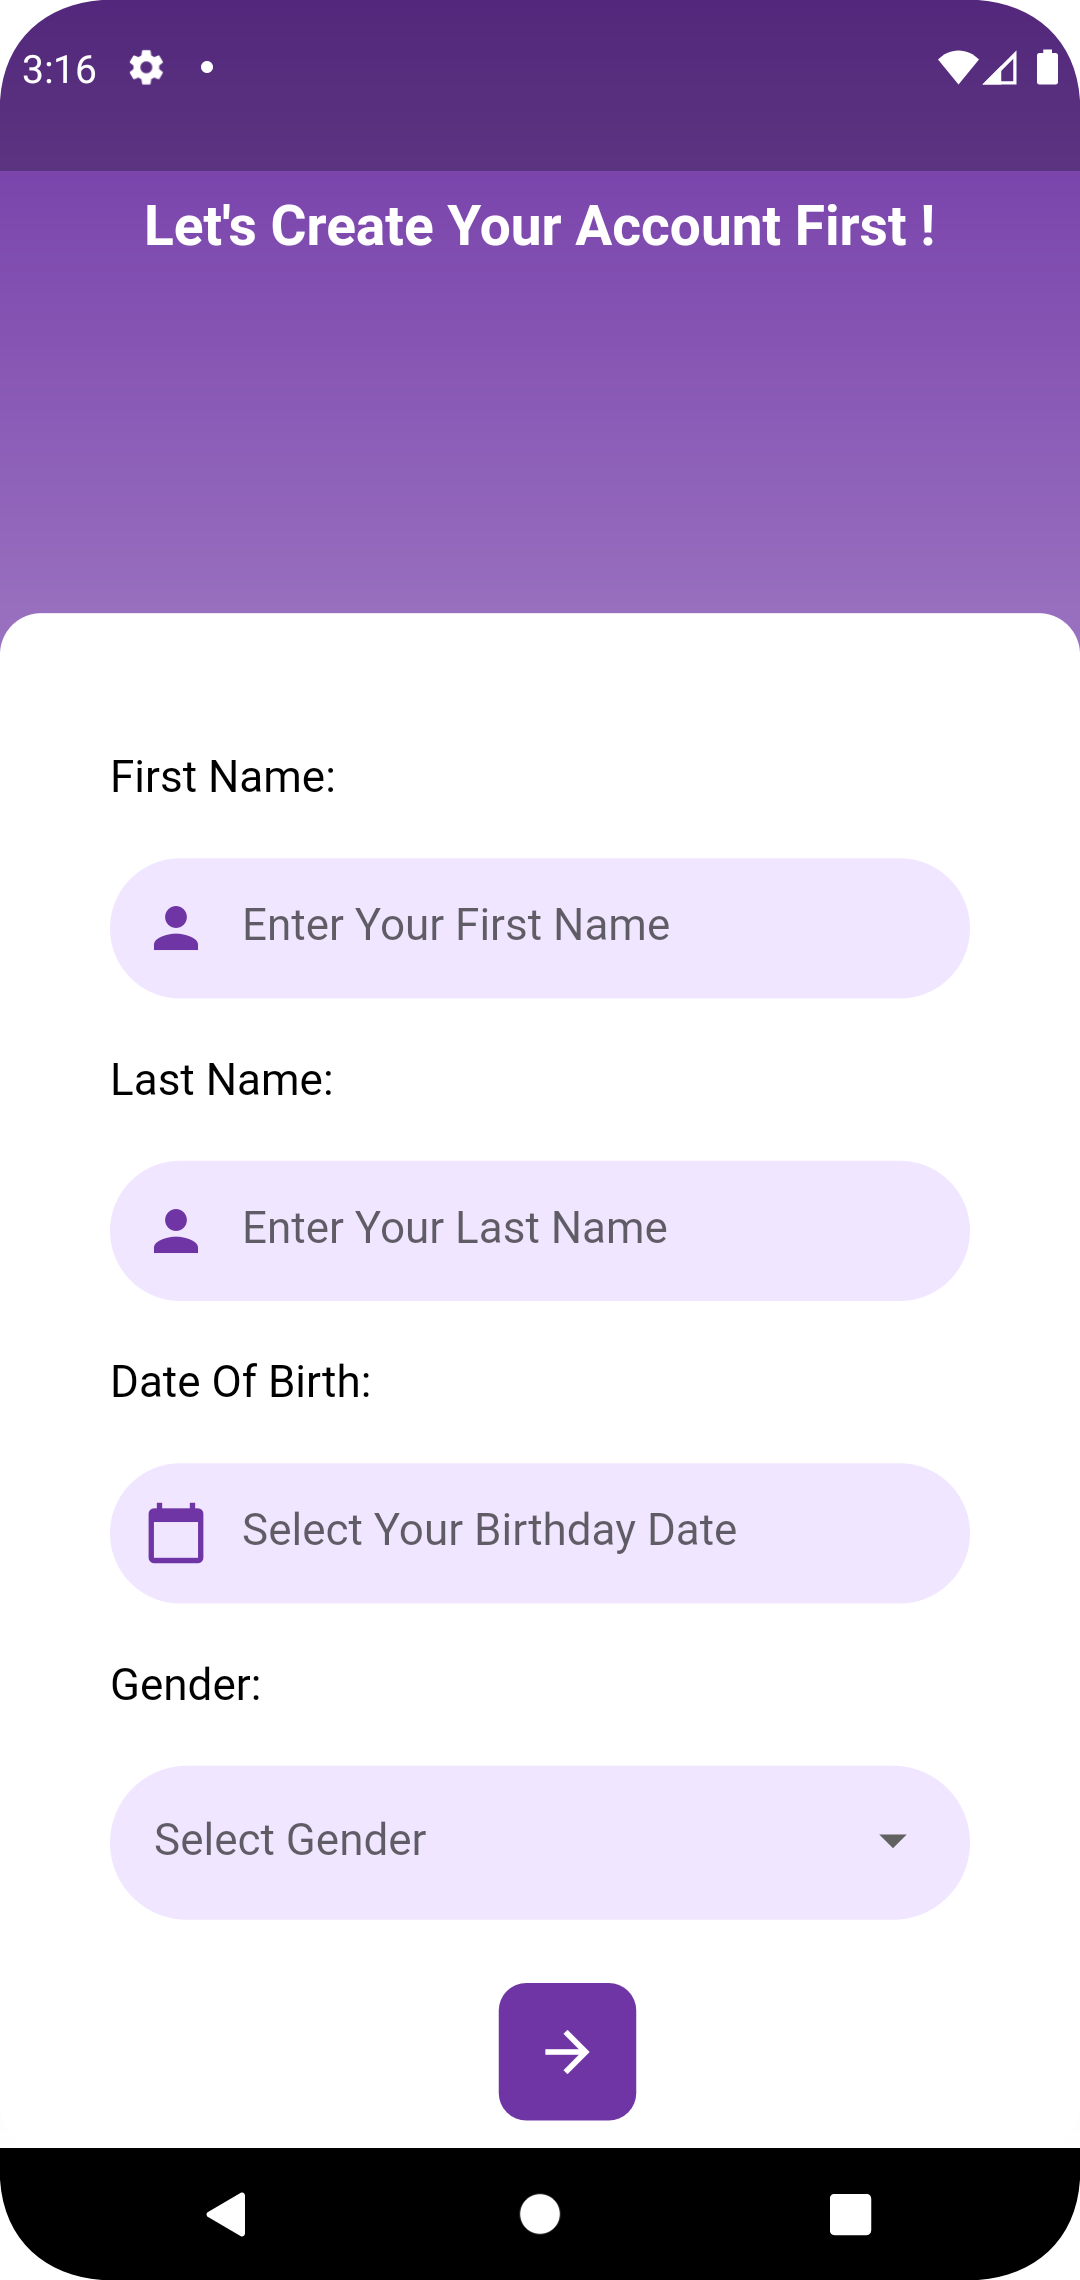
\includegraphics[height=9.5cm,width=7cm]{images/signup1.png}
        }
        \label{fig:second}
    \end{subfigure}
    
    \vspace{0.5cm}
    
    \begin{subfigure}{0.45\textwidth}
        \centering
        \setlength{\fboxsep}{5pt}%
        \setlength{\fboxrule}{0.5pt}%
        \fbox{
            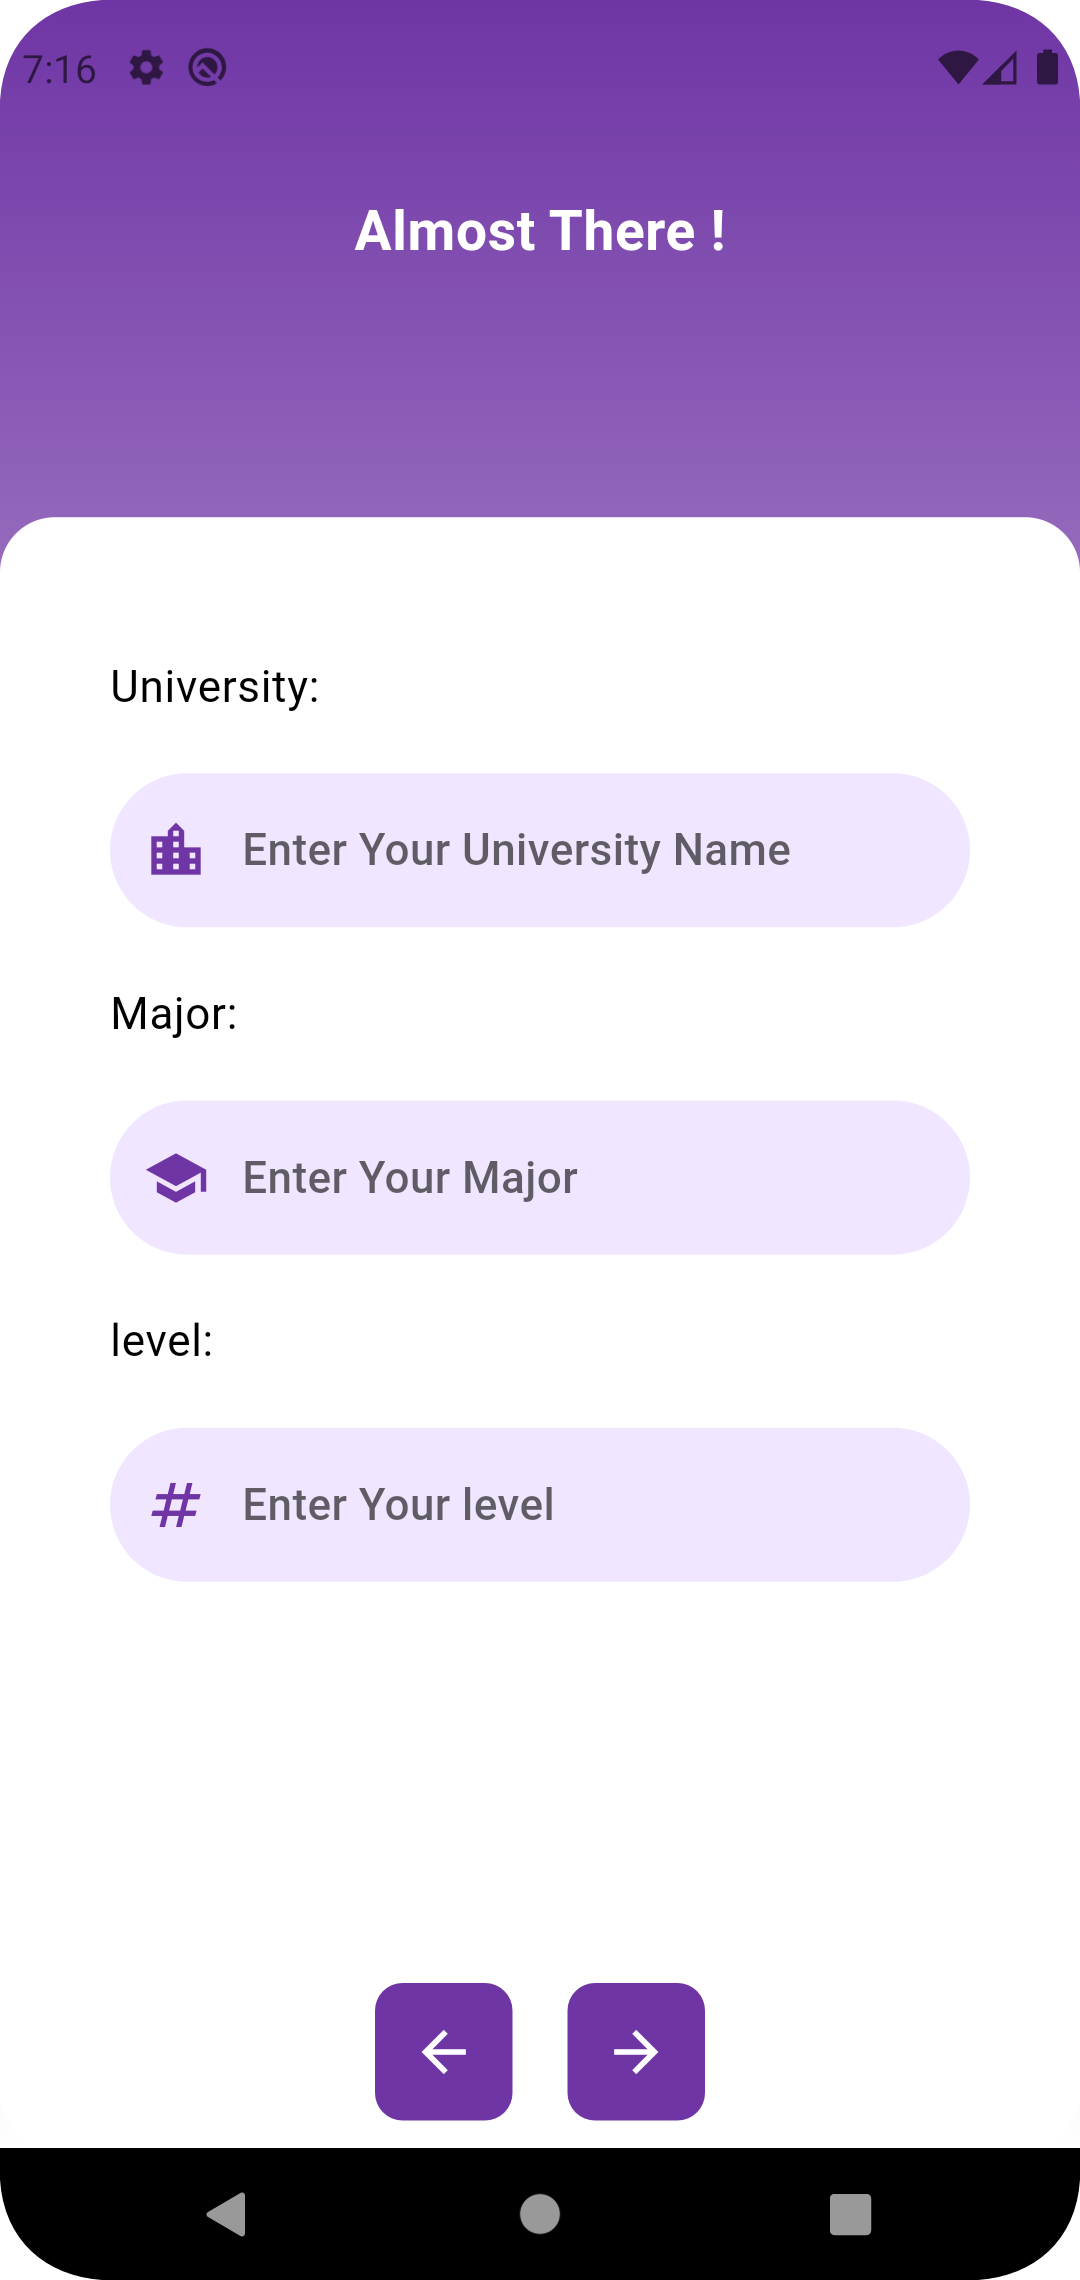
\includegraphics[height=9.5cm,width=7cm]{images/SignUpPage3.png}
        }
        \label{fig:third}
    \end{subfigure}
    \hfill
    \begin{subfigure}{0.45\textwidth}
        \centering
        \setlength{\fboxsep}{5pt}%
        \setlength{\fboxrule}{0.5pt}%
        \fbox{
            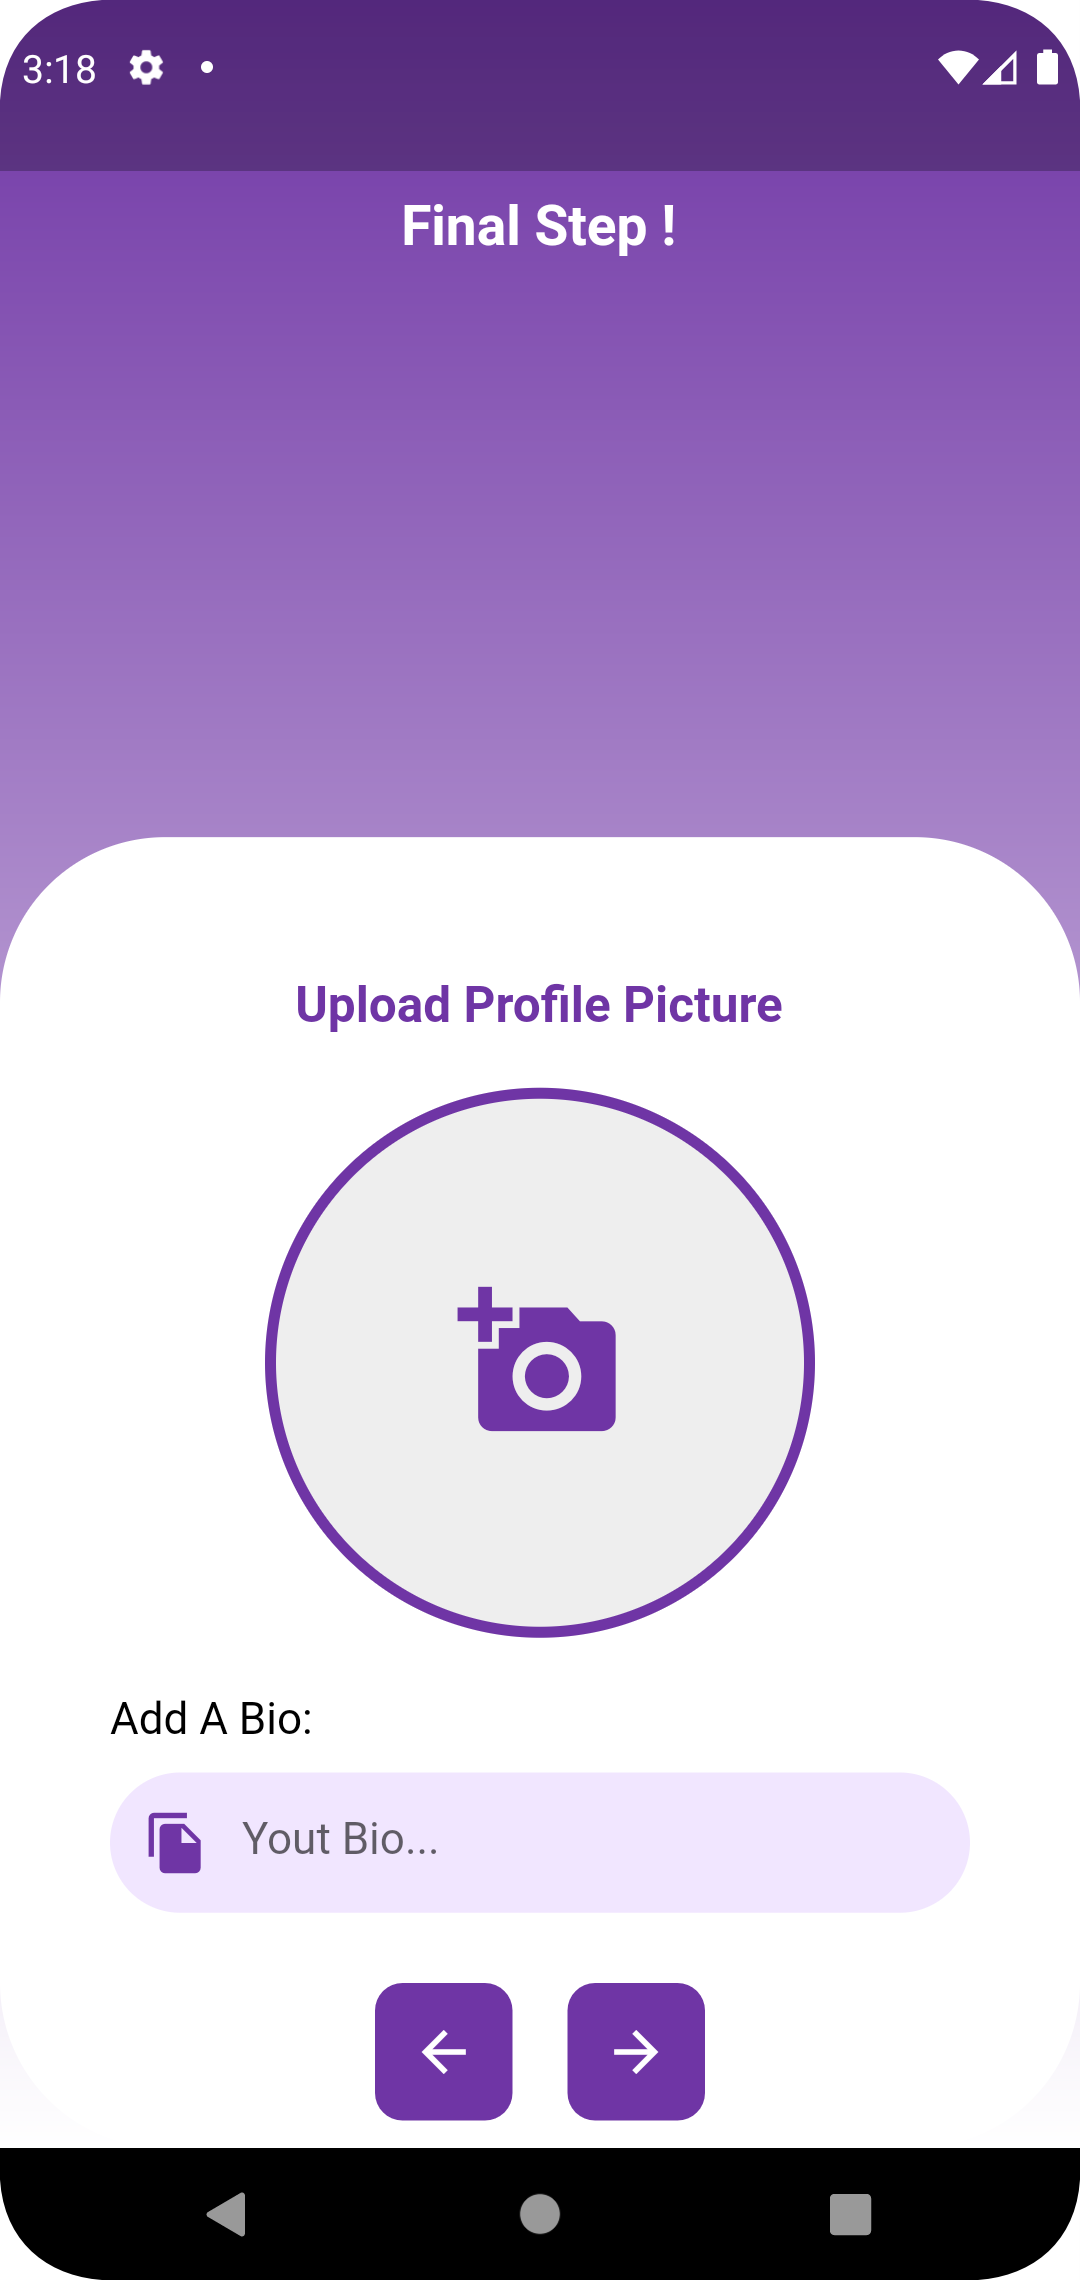
\includegraphics[height=9.5cm,width=7cm]{images/signup3.png}
        }
        \label{fig:fourth}
    \end{subfigure}

    \caption{Les Interfaces du formulaire SignUp}
    \label{fig:all}
\end{figure}



\newpage
\vspace{-8mm}
\subsection{Modifier profile}
\vspace{-6mm}
La page de modification du profil permet aux utilisateurs de mettre à jour leurs informations personnelles en quelques étapes simples, assurant ainsi l'exactitude des données de leur compte.
\vspace{-10mm}
\begin{figure}[H]%
    \center%
    \setlength{\fboxsep}{5pt}%
    \setlength{\fboxrule}{0.5pt}%
    \fbox{
    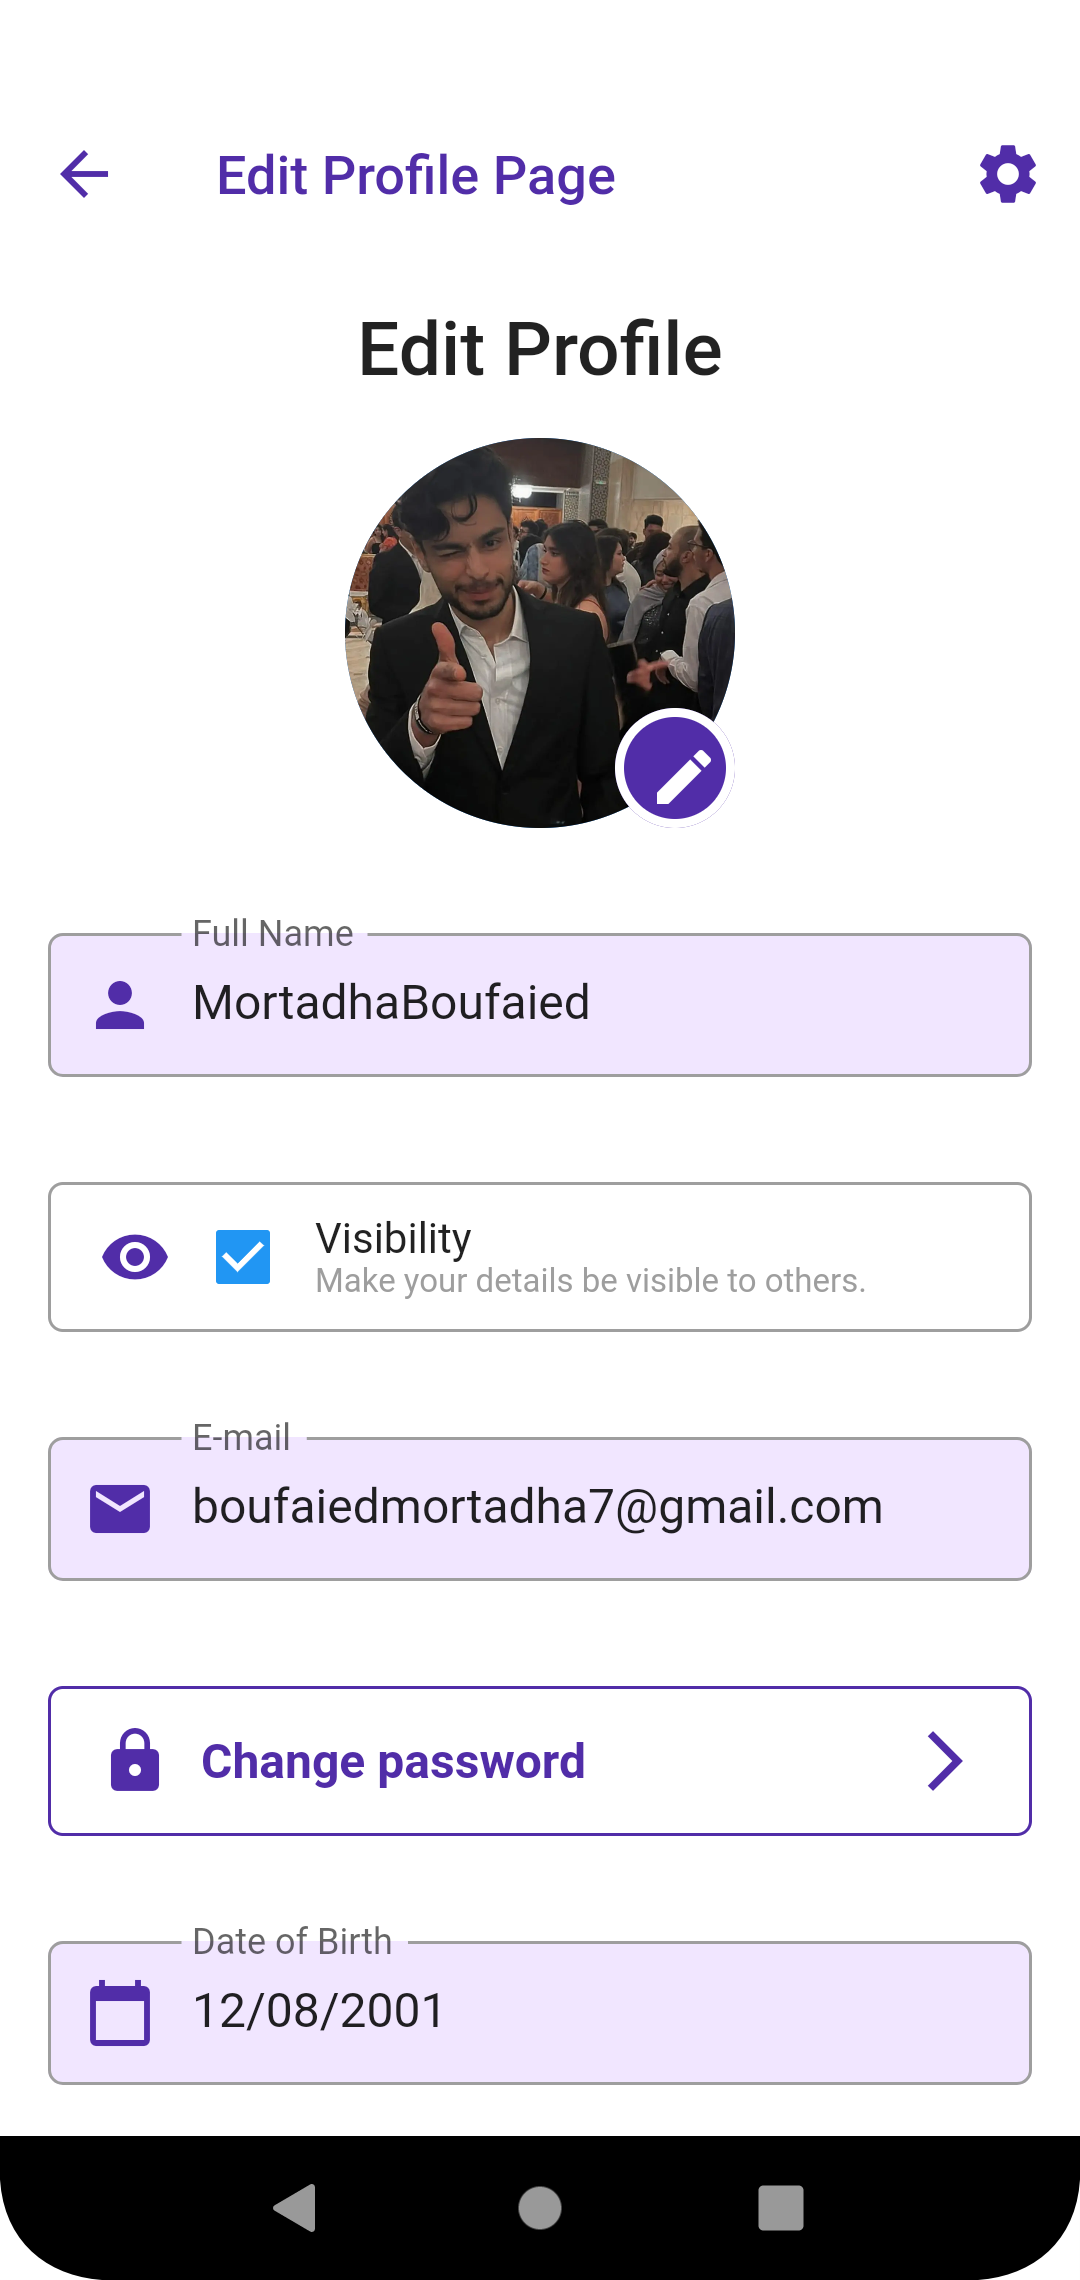
\includegraphics[height=9cm,width=7cm]{images/AAAEditProfile.png}%
    }
    \caption{Interface modifier profile }
\end{figure}
\vspace{-1.8cm}

\subsection{Changer mot de passe}
\vspace{-6mm}
La page permet de changer le mot de passe rapidement pour sécuriser le compte.
\vspace{-2mm}
\begin{figure}[H]%
    \center%
    \setlength{\fboxsep}{5pt}%
    \setlength{\fboxrule}{0.5pt}%
    \fbox{
    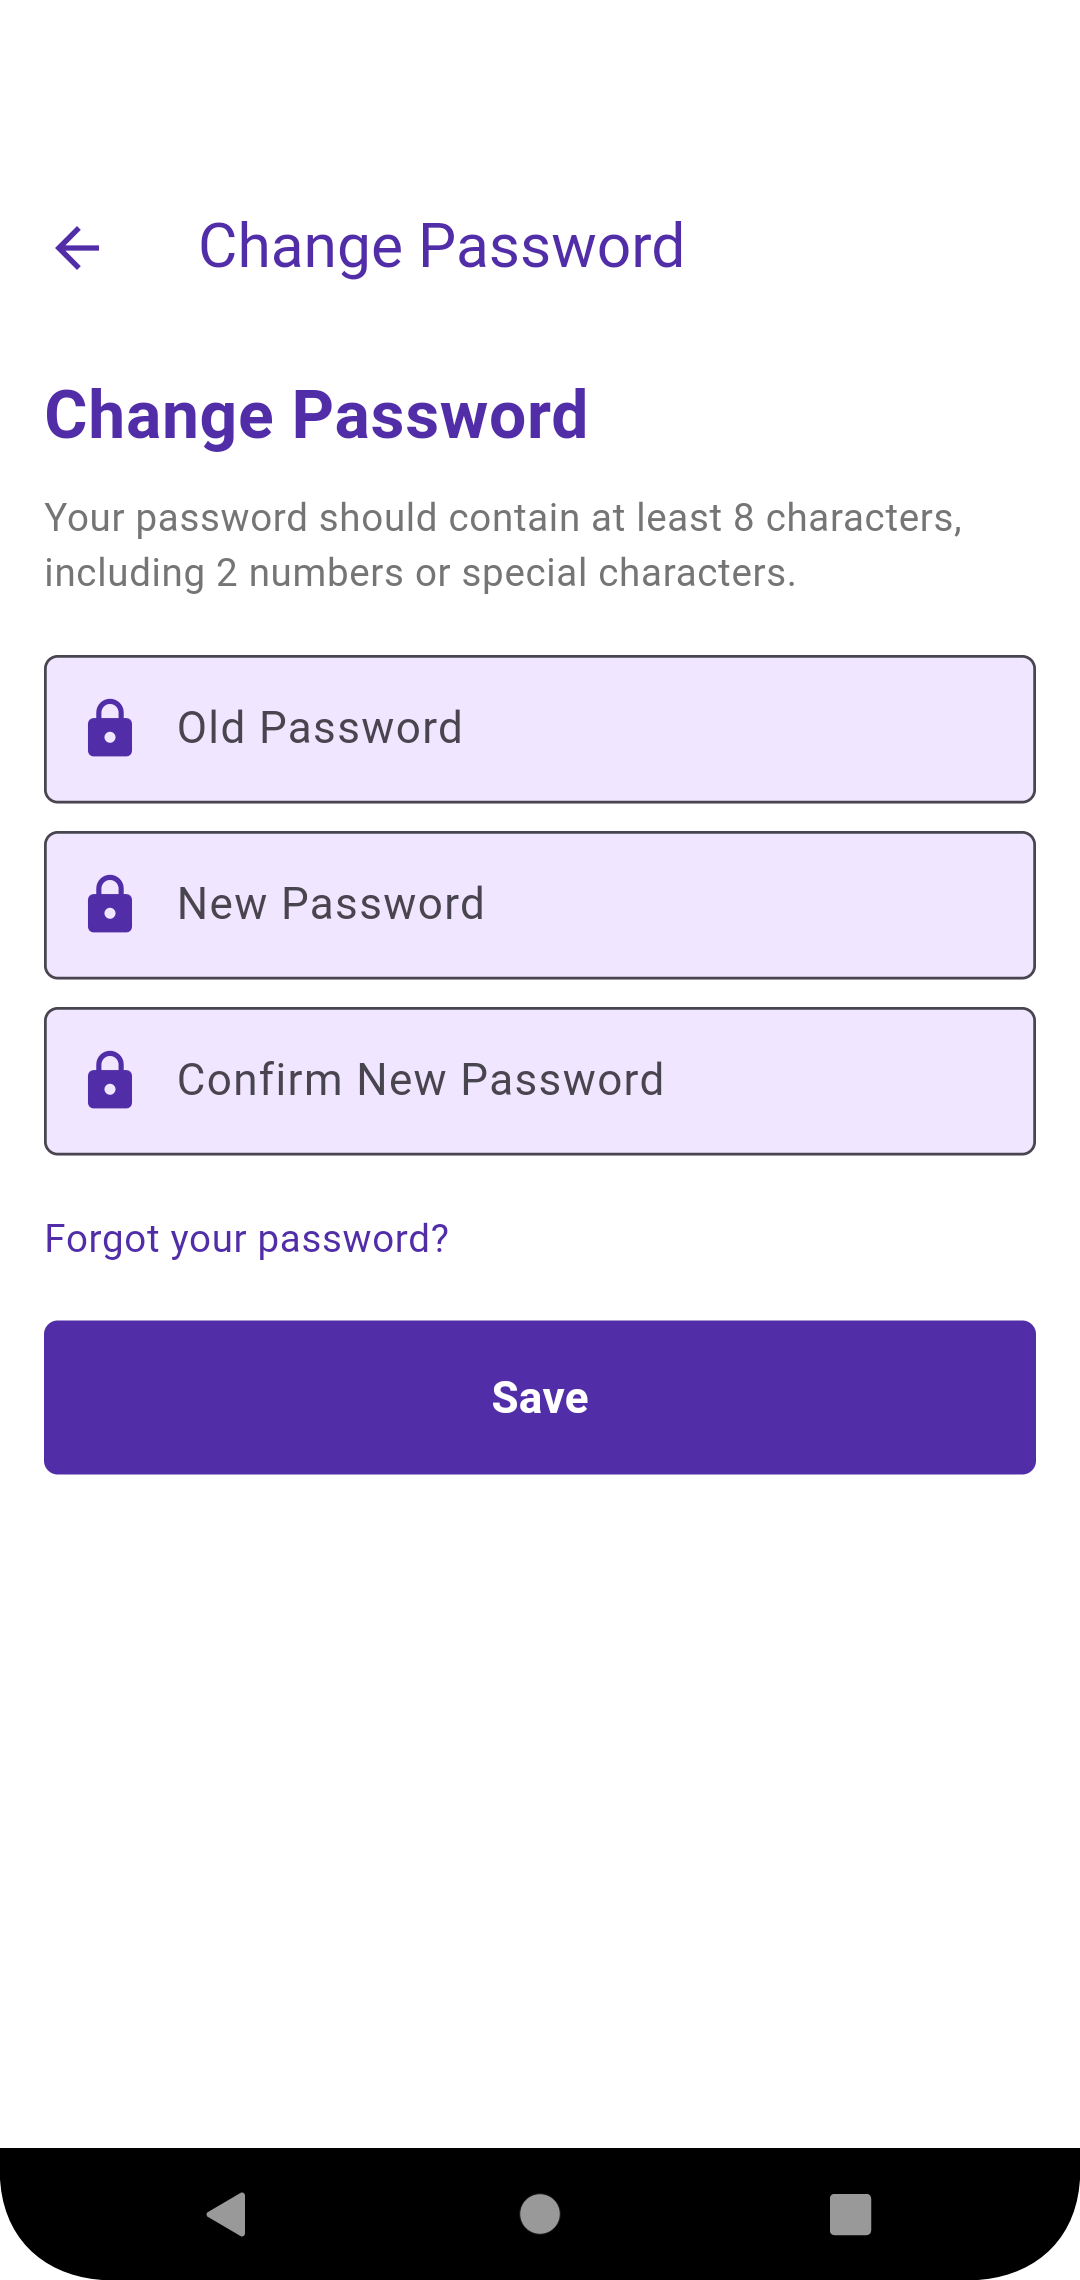
\includegraphics[height=9cm,width=7cm]{images/ChangePassword.png}%
    }
    \caption{Interface changer mot passe }
\end{figure}

\vspace{-4mm}

\subsection{Réinitialiser mot de passe}
\vspace{-4mm}
La réinitialisation du mot de passe permet aux utilisateurs de regagner l'accès à leur compte en cas d'oubli. Ils reçoivent un lien par e-mail pour réinitialiser leur mot de passe et choisir un nouveau en quelques clics.
\begin{figure}[H]
    \centering

    % Première ligne avec deux images côte à côte
    \begin{subfigure}{0.45\textwidth}
        \centering
        \setlength{\fboxsep}{5pt}%
        \setlength{\fboxrule}{0.5pt}%
        \fbox{
            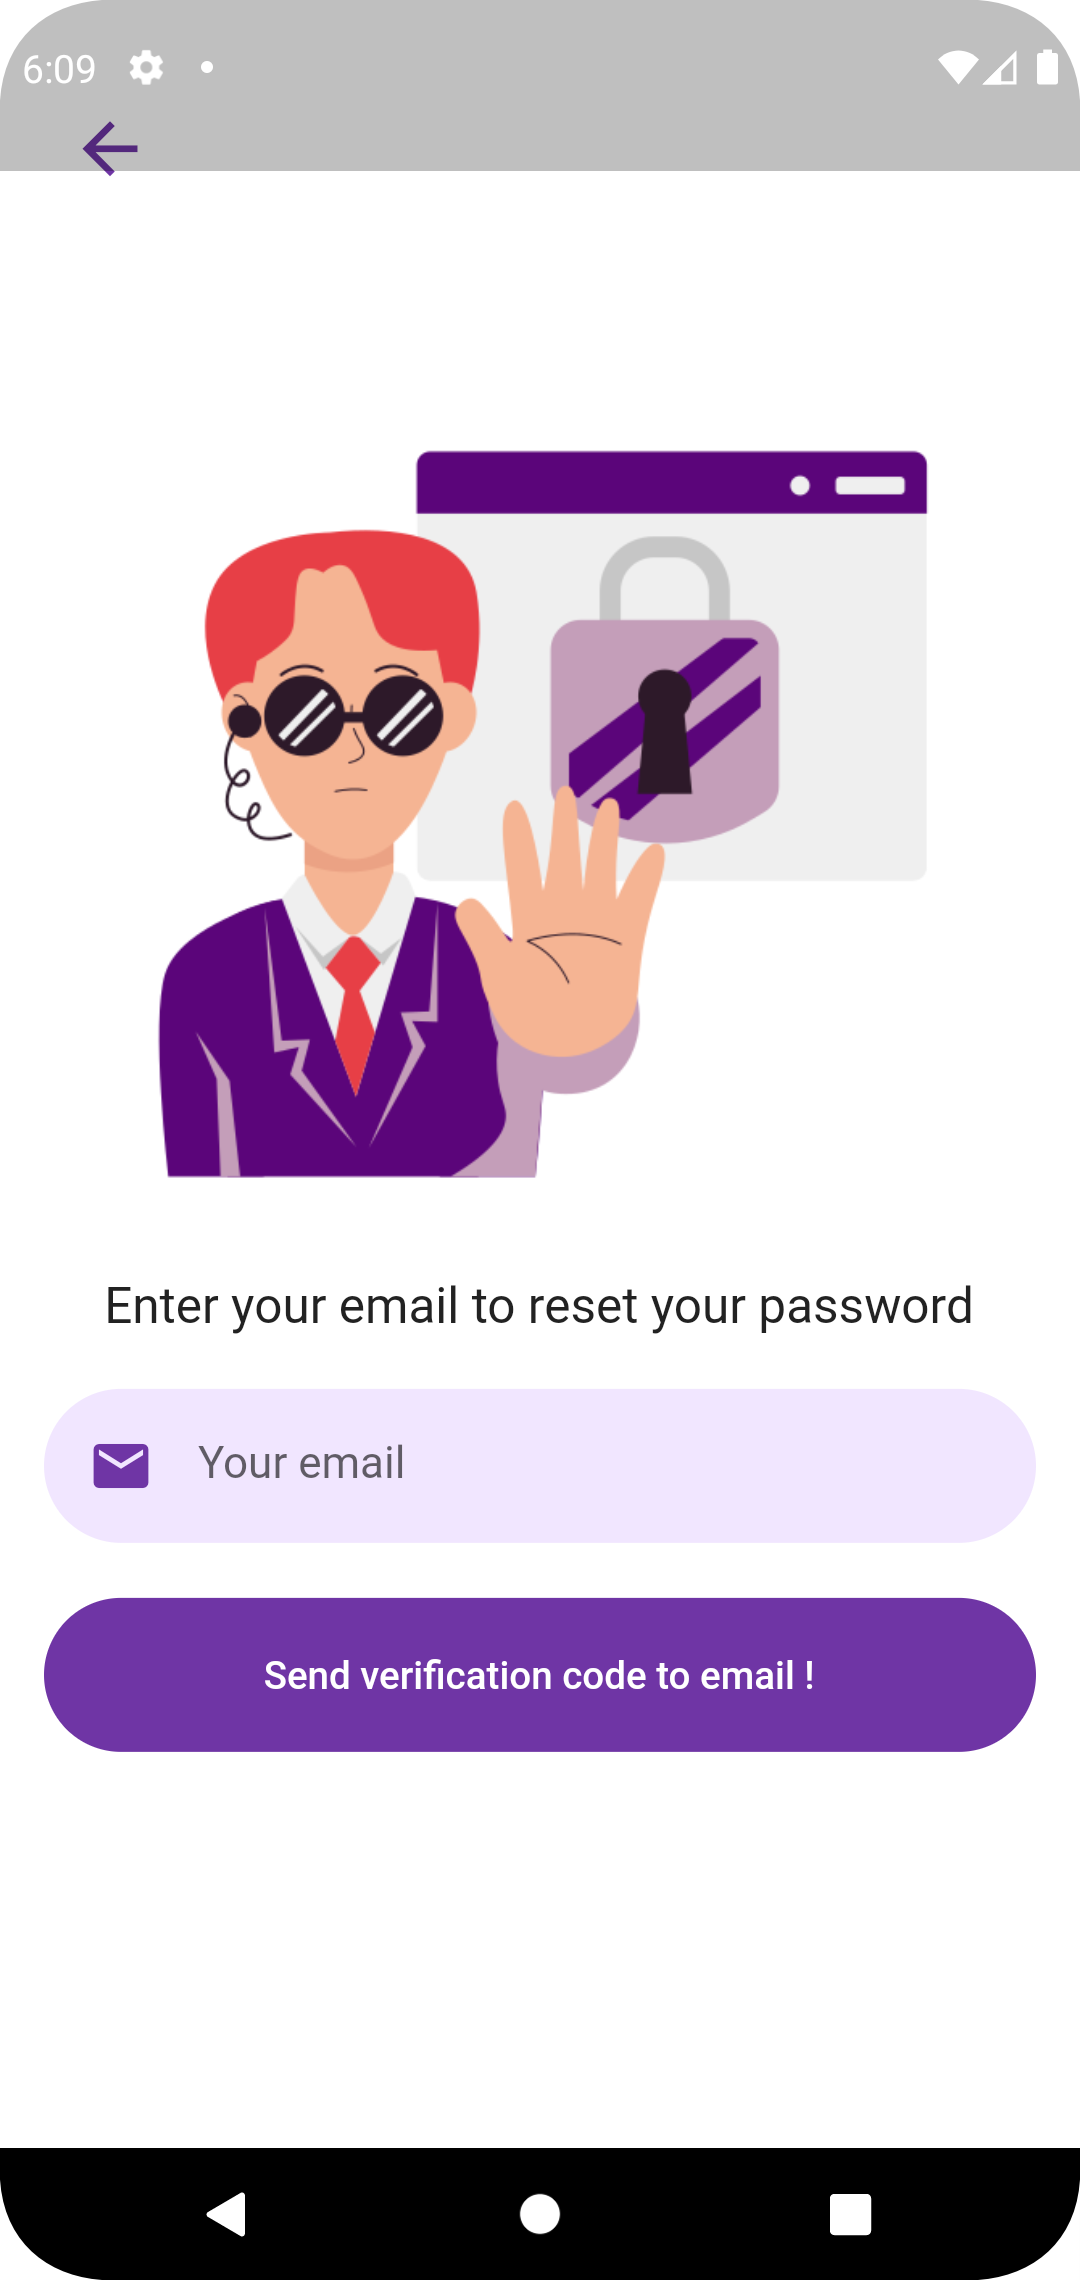
\includegraphics[height=9.2cm,width=7cm]{images/ForgetPassword1.png}
        }
        \label{fig:first}
    \end{subfigure}
    \hfill
    \begin{subfigure}{0.45\textwidth}
        \centering
        \setlength{\fboxsep}{5pt}%
        \setlength{\fboxrule}{0.5pt}%
        \fbox{
            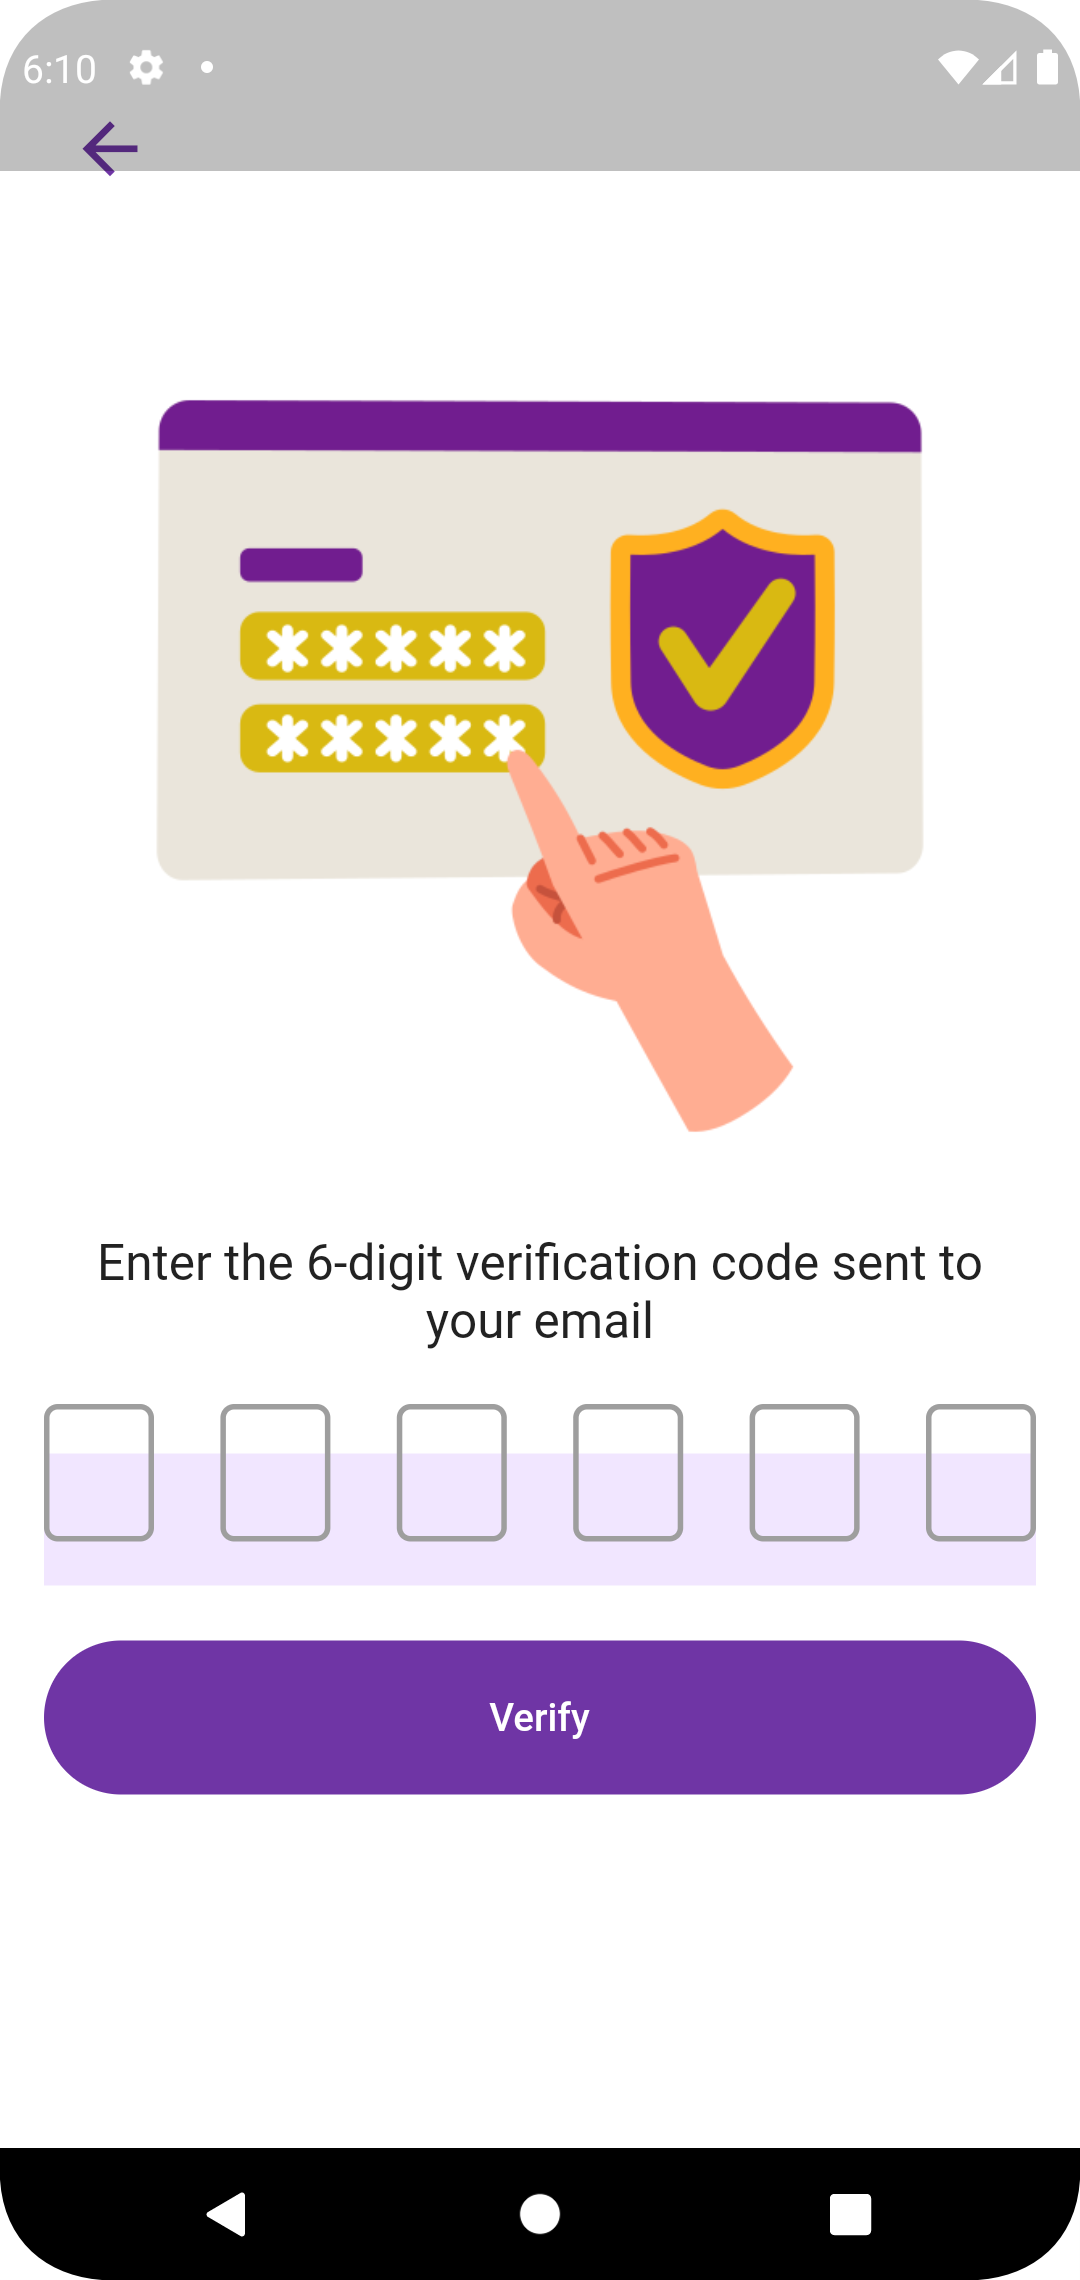
\includegraphics[height=9.2cm,width=7cm]{images/ForgetPassword2.png}
        }
        \label{fig:second}
    \end{subfigure}
    
    \vspace{-0.2cm}

    % Deuxième ligne avec une seule image centrée
    \begin{subfigure}{0.45\textwidth}
        \centering
        \setlength{\fboxsep}{5pt}%
        \setlength{\fboxrule}{0.5pt}%
        \fbox{
            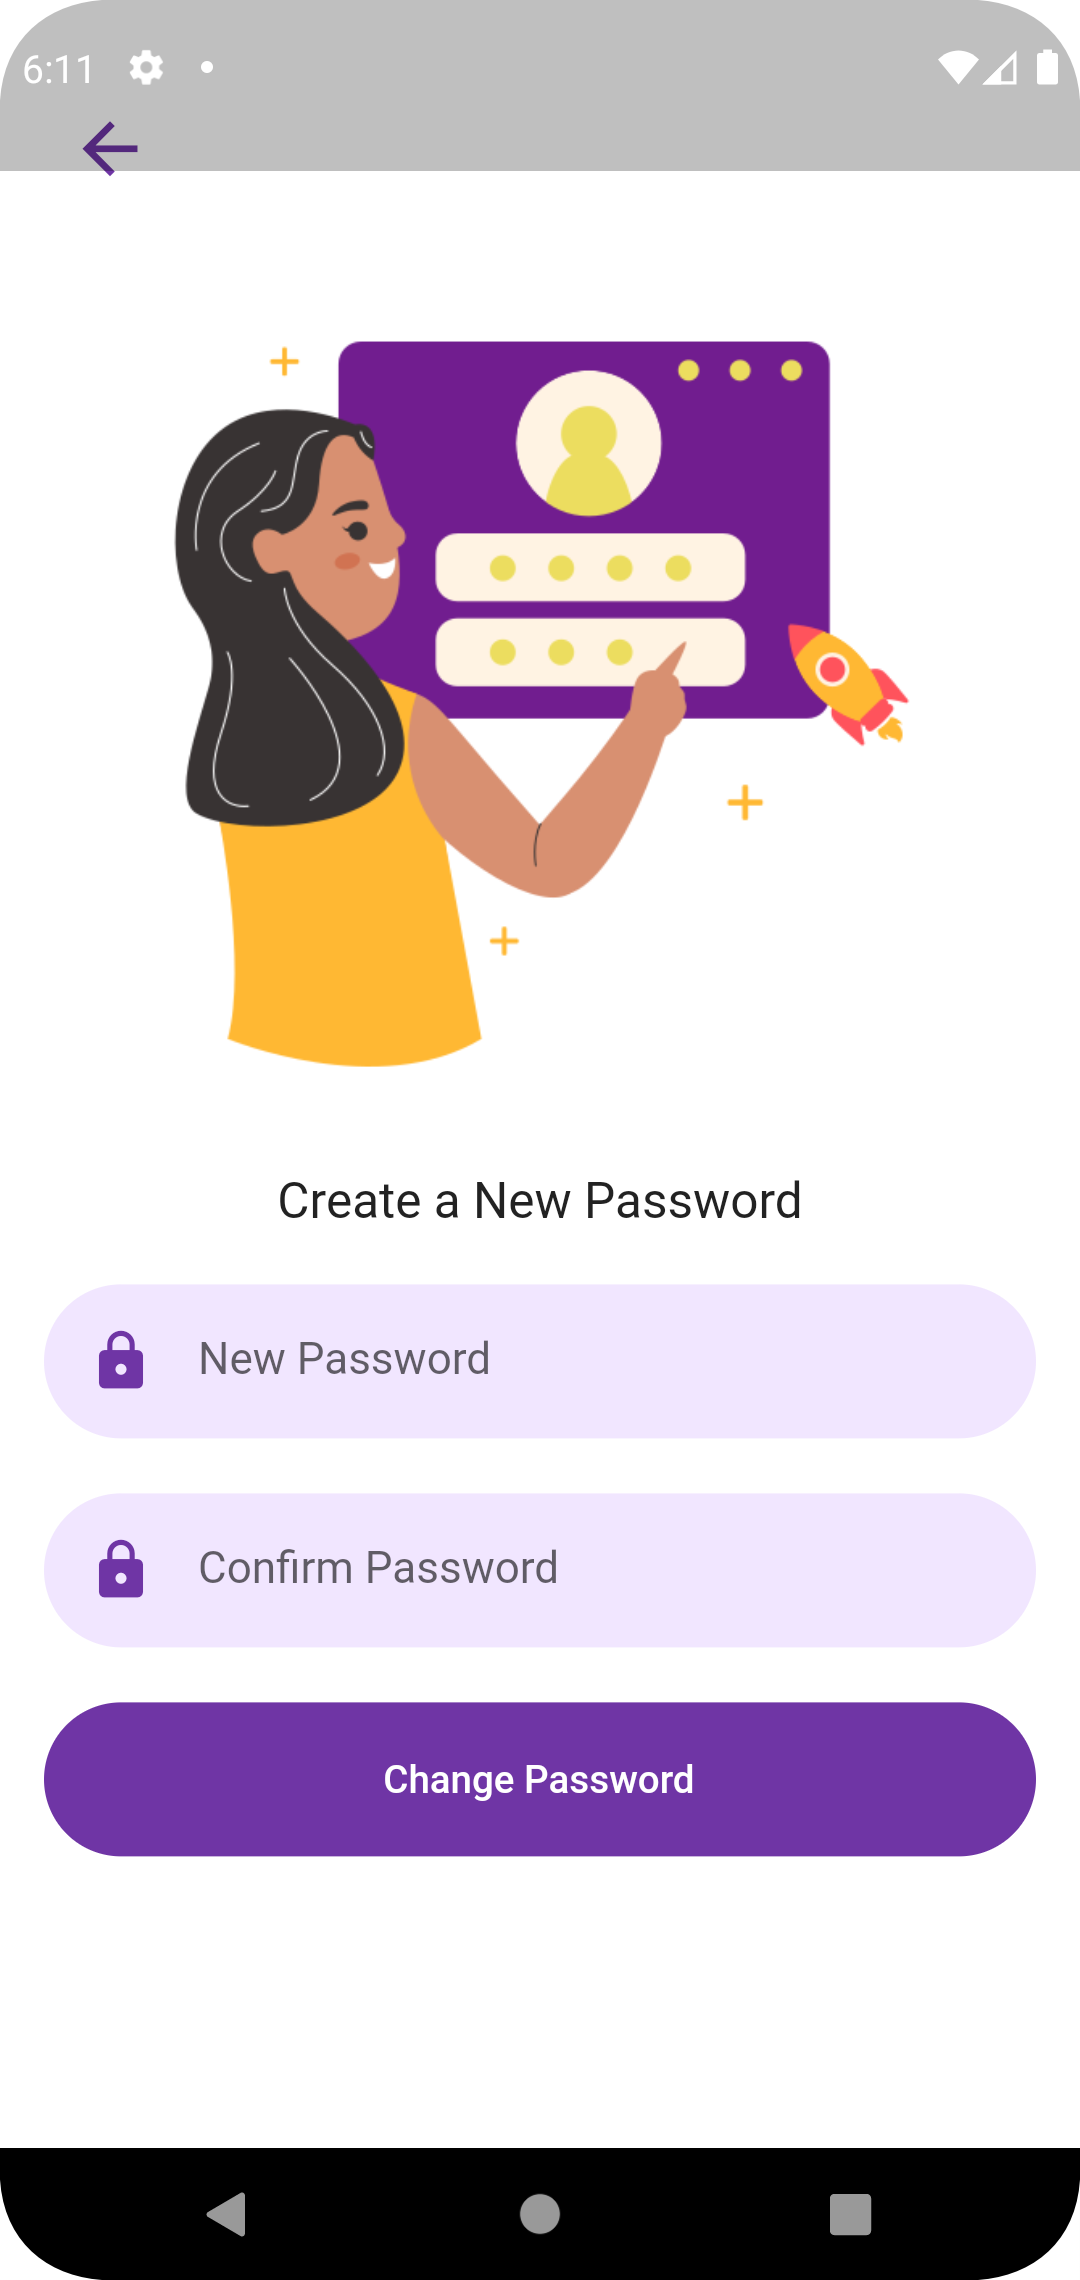
\includegraphics[height=9.2cm,width=7cm]{images/ForgetPassword3.png}
        }
        \label{fig:third}
    \end{subfigure}
    \vspace{-4mm}
    \caption{Les interfaces de la page de mot de passe oublié}
    \label{fig:three}
\end{figure}


\vspace{-4mm}
\subsection{Page Profile}
\vspace{-4mm}
La page de profil utilisateur permet aux utilisateurs de visualiser et de modifier leurs informations personnelles, ainsi que de consulter les publications qu'ils ont créées et les images qu'ils ont partagées.
\begin{figure}[H]
    \centering

    % Première ligne avec deux images côte à côte
    \begin{subfigure}{0.45\textwidth}
        \centering
        \setlength{\fboxsep}{5pt}%
        \setlength{\fboxrule}{0.5pt}%
        \fbox{
            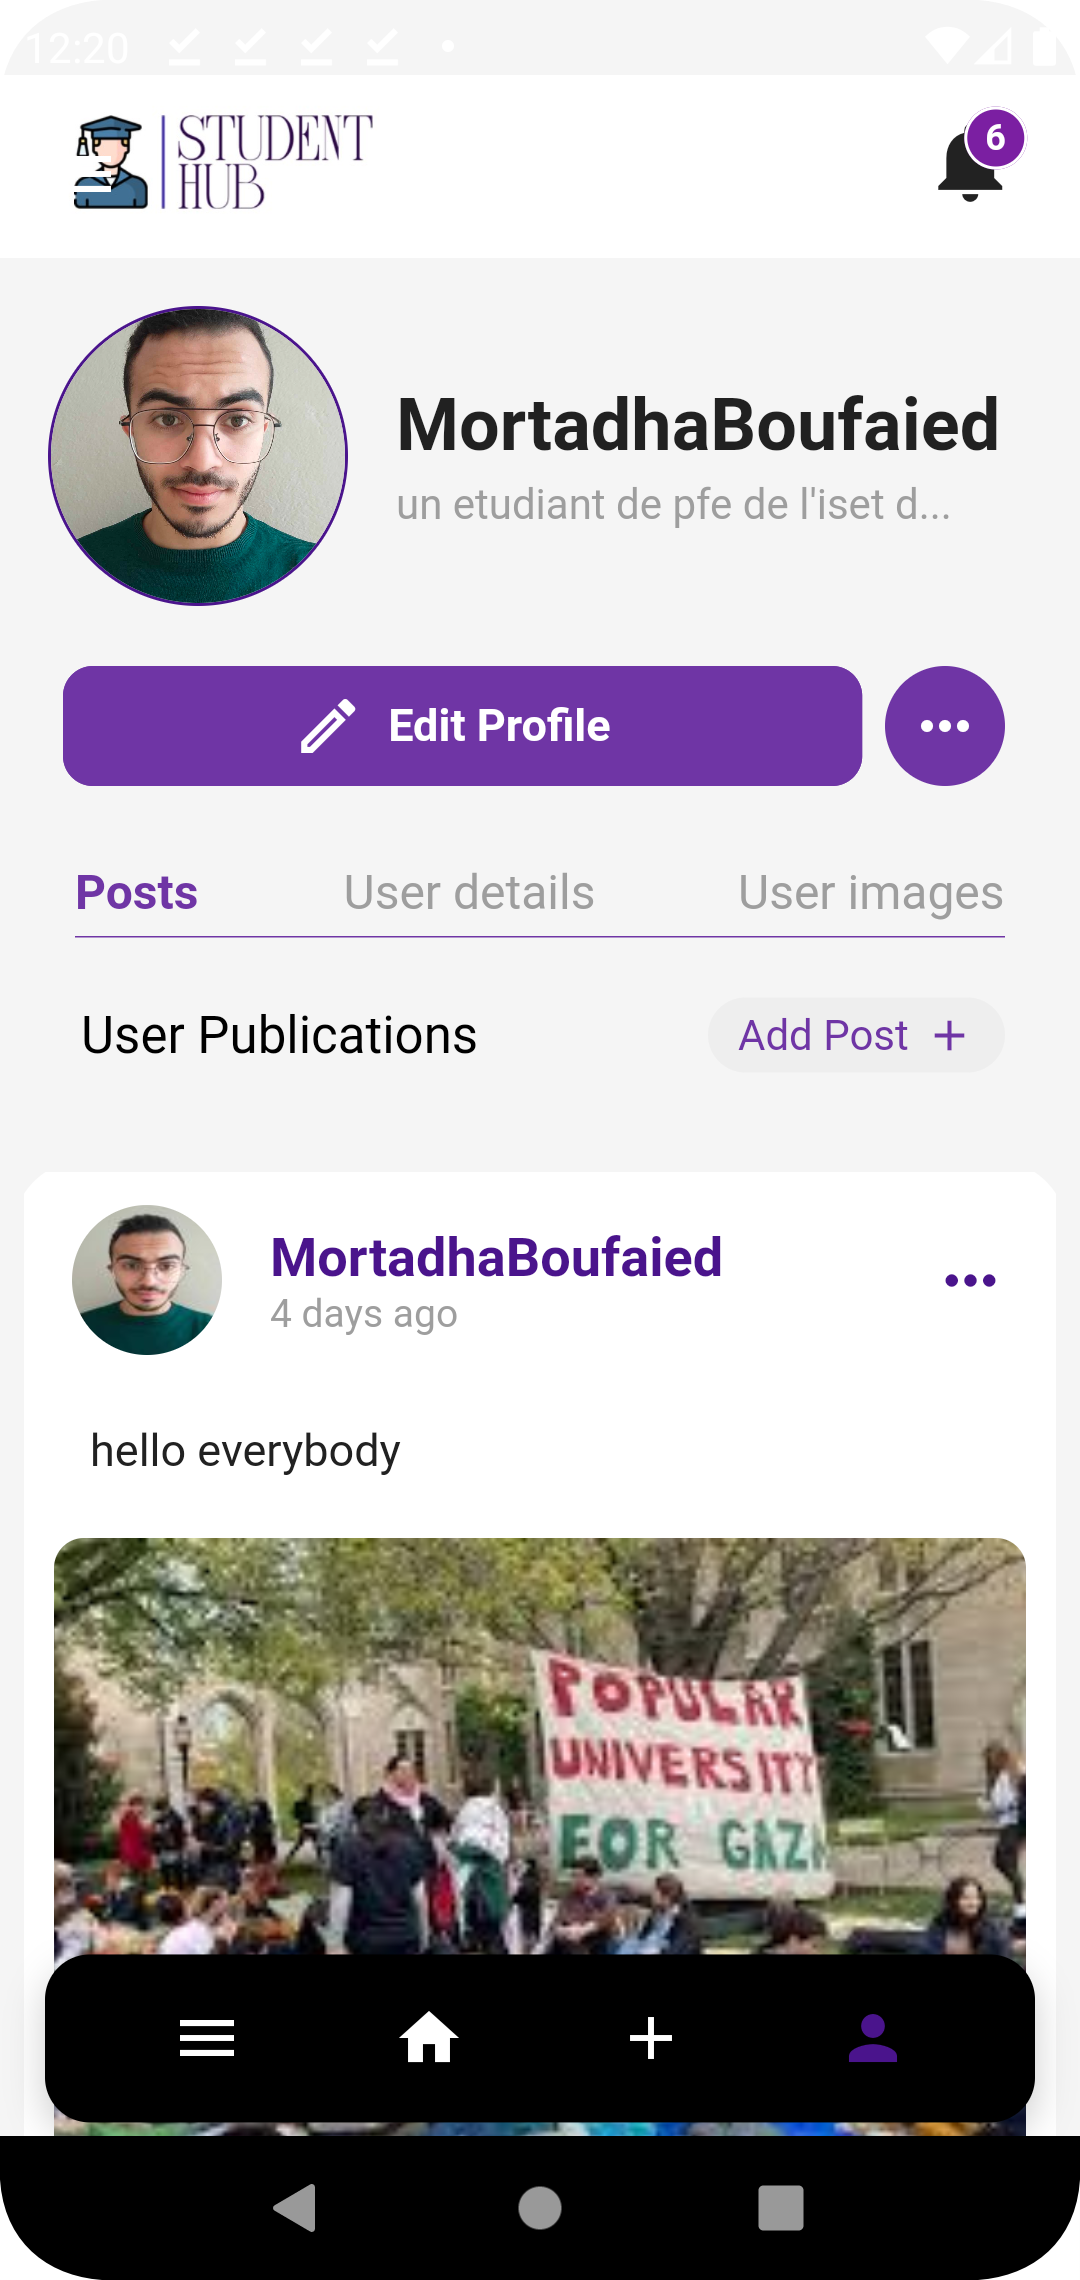
\includegraphics[height=9.2cm,width=7cm]{images/AAAProfile.png}
        }
        \label{fig:first}
    \end{subfigure}
    \hfill
    \begin{subfigure}{0.45\textwidth}
        \centering
        \setlength{\fboxsep}{5pt}%
        \setlength{\fboxrule}{0.5pt}%
        \fbox{
            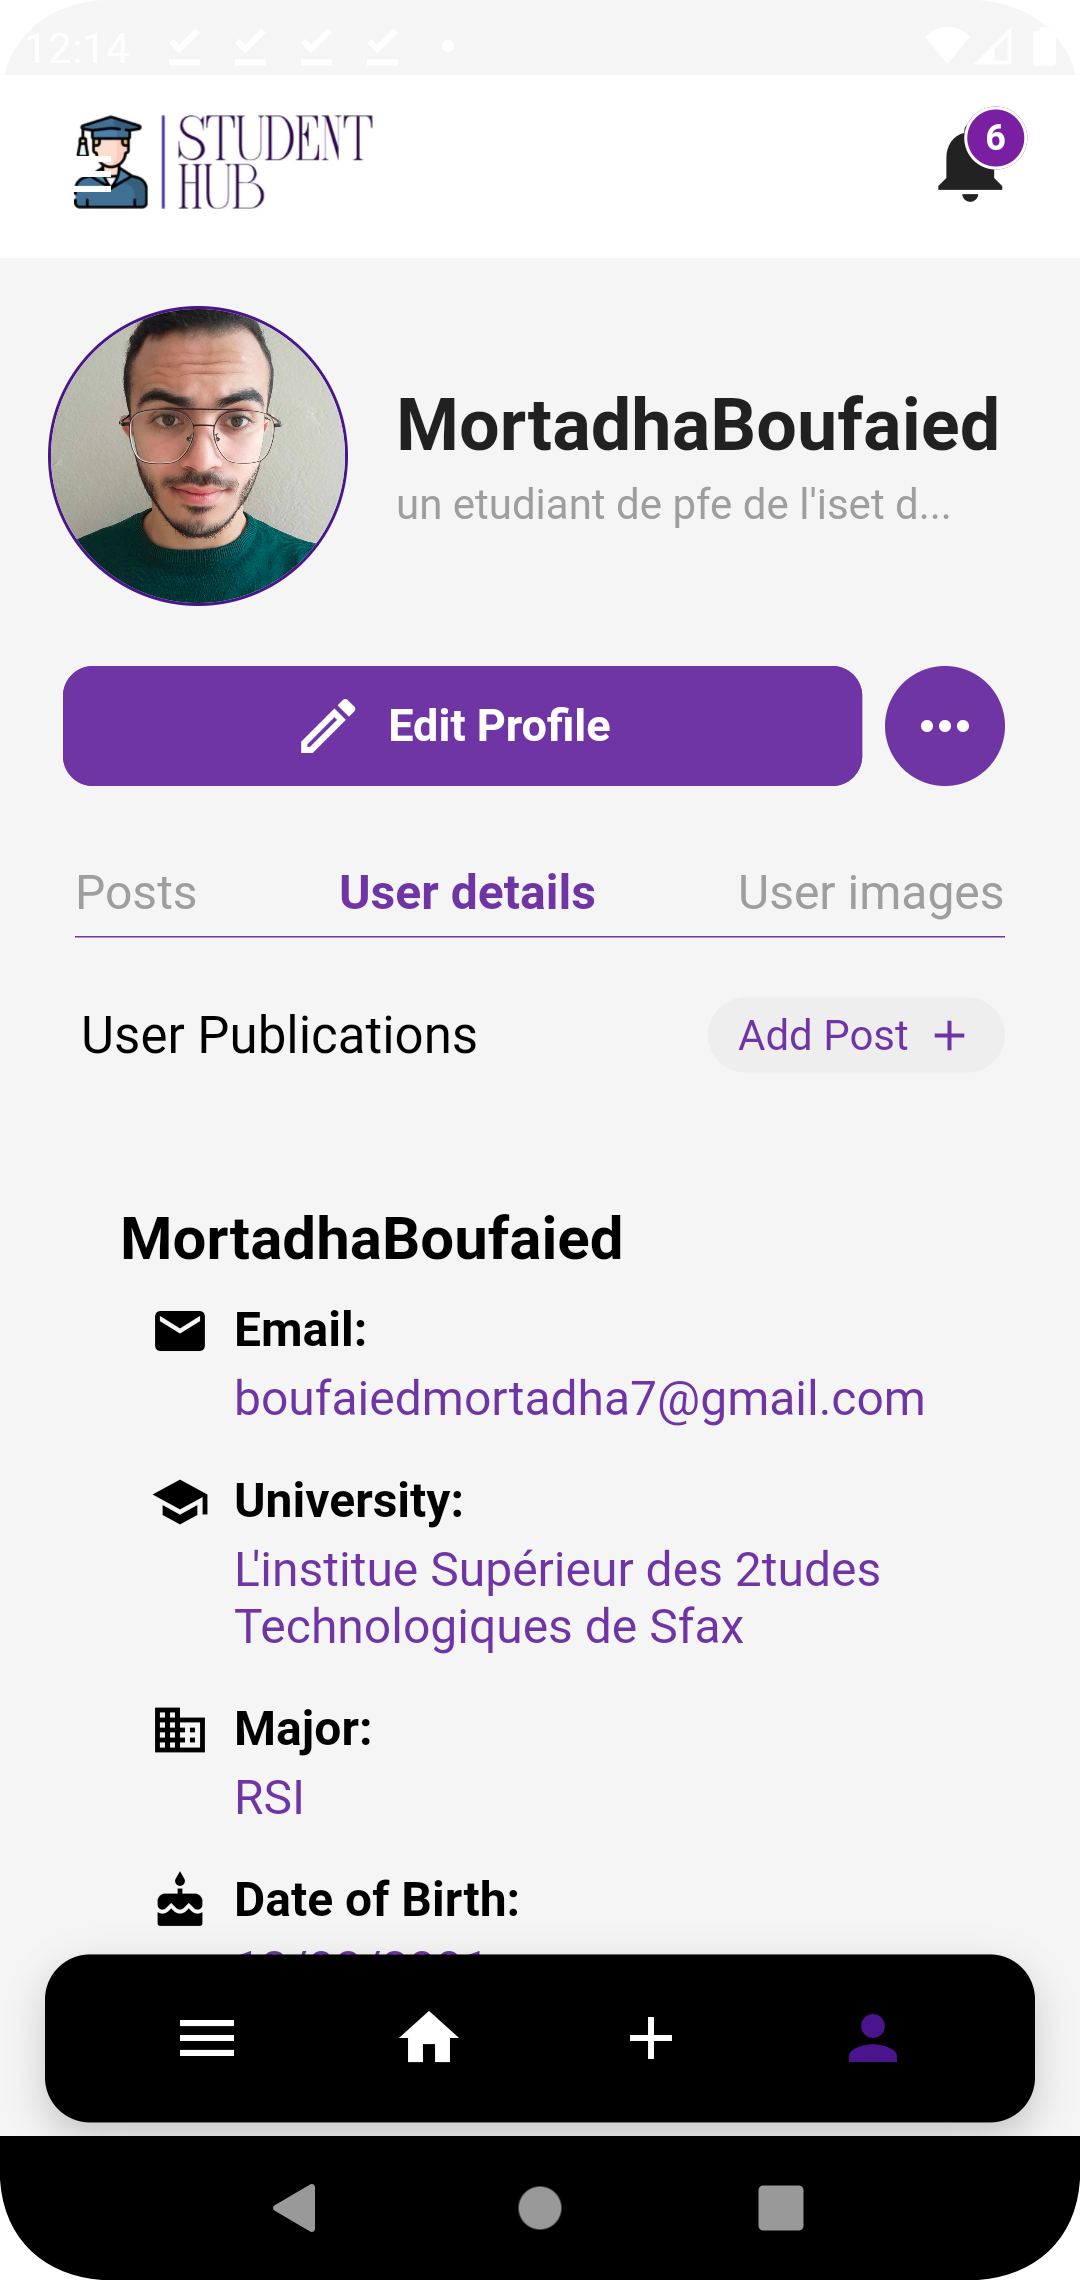
\includegraphics[height=9.2cm,width=7cm]{images/AAAUserDetails.png}
        }
        \label{fig:second}
    \end{subfigure}
    
    \vspace{-0.2cm}

    % Deuxième ligne avec une seule image centrée
    \begin{subfigure}{0.45\textwidth}
        \centering
        \setlength{\fboxsep}{5pt}%
        \setlength{\fboxrule}{0.5pt}%
        \fbox{
            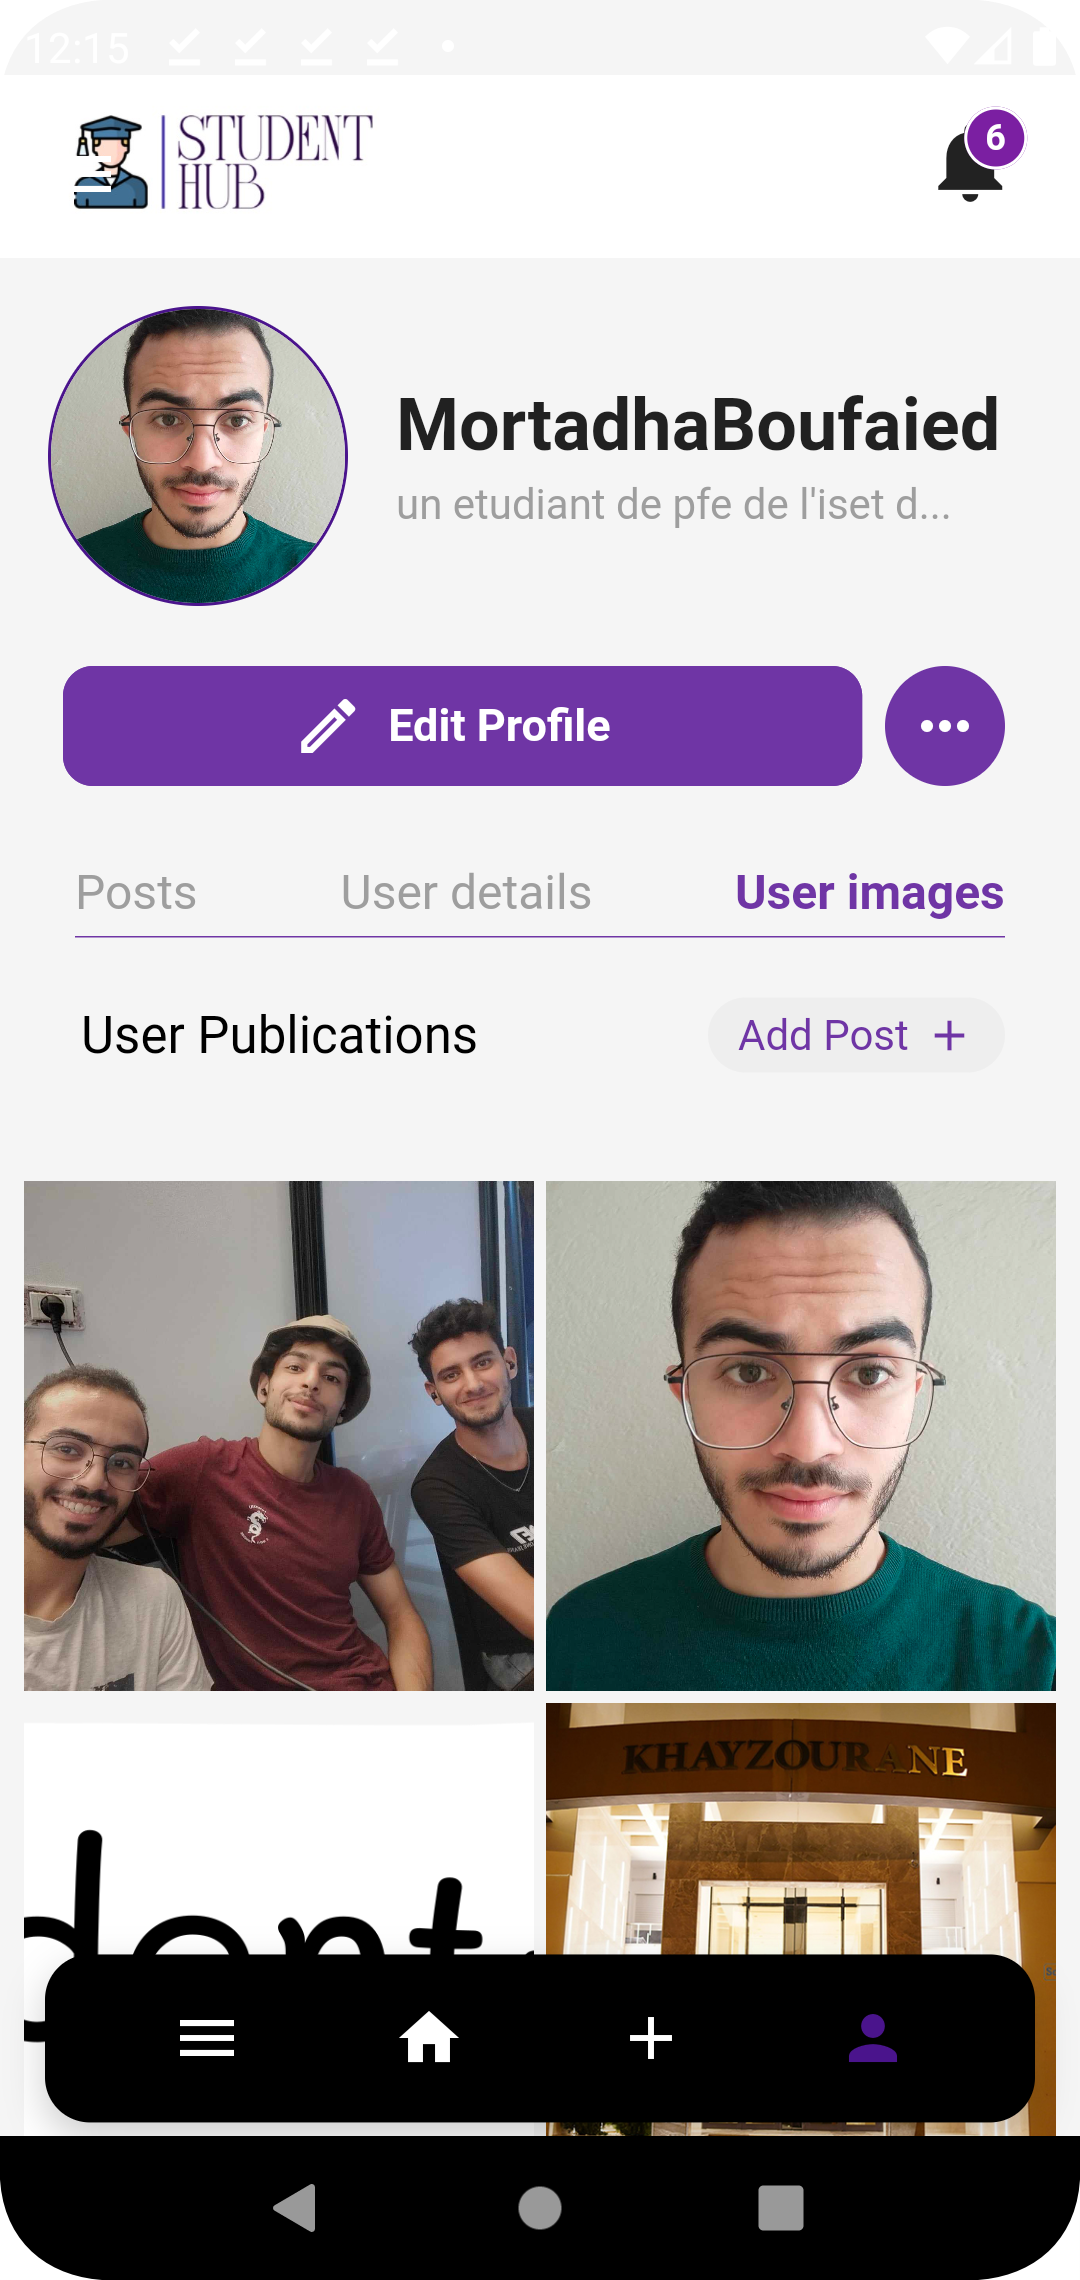
\includegraphics[height=9.2cm,width=7cm]{images/AAAUserImages.png}
        }
        \label{fig:third}
    \end{subfigure}
    \vspace{-5mm}
    \caption{Les interfaces du page profile}
    \label{fig:three}
\end{figure}

\vspace{-4mm}
\newpage
\section{Conclusion }
\vspace{-4mm}
Ce premier sprint a été essentiel pour mettre en place les fonctionnalités de base de notre système. Nous avons réussi à mettre en œuvre la création de comptes, l'authentification, la gestion des utilisateurs, ainsi que la réinitialisation des mots de passe. Ces fonctionnalités constituent la fondation de notre application, et nous permettront de fournir une expérience utilisateur fluide et sécurisée.. Nous passons maintenant vers le chapitre suivant qui est consacré au Sprint 2.

\end{sloppypar}


